\documentclass[11pt,a4paper]{article}
\usepackage[margin=1in, paperwidth=8.5in, paperheight=11in]{geometry}

\usepackage{ifxetex}

\ifxetex
  \usepackage{fontspec}
  \usepackage{polyglossia}
  \setdefaultlanguage{polish}
\else
  \usepackage{polski}
  \usepackage[T1]{fontenc}
  \usepackage[utf8]{inputenc}
  \usepackage{lmodern}
  \usepackage[polish]{babel}
\fi

\usepackage{indentfirst}
\usepackage{parskip}
\usepackage{rotating}
\usepackage[hidelinks]{hyperref}
\usepackage[table]{xcolor}
\usepackage{float}
\usepackage{hhline}
\usepackage{multirow}
\usepackage{amsmath}
\usepackage{amsfonts}
\usepackage{titlesec}
\usepackage{tabularx}
\usepackage{listings}

\newcommand{\sectionbreak}{\clearpage}

\setlength{\parindent}{12pt}
%\setlength{\parskip}{1,0em}

\graphicspath{ {img/} }

\setcounter{tocdepth}{1}

\title{Opracowanie zagadnień z obrony inżynierskiej ze specjalności: INT, INS}
\author{}
\newcommand{\University}{Politechnika Wrocławska}
\newcommand{\Department}{Wydział Elektroniki}
\newcommand{\Faculty}{Informatyka}


\makeatletter
\renewcommand{\maketitle}{
\begin{titlepage}
    \begin{center}
        %\vspace*{0.5cm}
        \huge\textsc{{\University}}\\
        \Large\textsc{{\Department}}\\
        \Large\textsc{{\Faculty}}\par
        
        \vspace{5cm}
        \huge\textbf{\@title}\par
        
        \vspace{5cm}
        \large\textit{Autorzy:}\\ 
        \Large\textbf{\@author}\par 
        
        \vspace{4cm}
        \small Wrocław \\
        \small \@date \\
    \end{center}
\end{titlepage}
}
\makeatother

\begin{document}
\tableofcontents
\newpage

\part{Pytania kierunkowe}
\section{K1 - Paradygmat programowania obiektowego}

Programowanie obiektowe stanowi podejście do implementacji algorytmów, które opiera się na wykorzystaniu tak zwanych \textbf{obiektów.} Są to twory, które łączą w sobie dane oraz zachowania oraz komunikują się ze sobą w celu wykonania pewnych zadań.

Paradygmat ten ma stanowić ułatwienie w pisaniu i utrzymywaniu kodu, który może być używany wielokrotnie w różnych projektach.

Pojęciami, na których się skupię będą:
\begin{itemize}
	\item Klasa
	\item Abstrakcja
	\item Enkapsulacja
	\item Dziedziczenie
	\item Polimorfizm
\end{itemize}

\textbf{Klasa} stanowi pewien zbiór cech i zachowań danego obiektu, który jest jej instancją.

Przykładem może być klasa \textit{Pies,} która zawiera cechy takie jak oczy, pysk oraz umiejętność szczekania.

\textbf{Abstrakcja,} czyli poziom ogólności, pozwala nam na upraszczanie problemu poprzez zredukowanie właściwości do jedynie tych kluczowych dla algorytmu.

Dla przykładu - możemy mówić o \textit{Bazie danych} jako o fragmencie kodu, który będzie stanowił interfejs do komunikacji z pewną bazą danych, jednak nie ma to dla nas większego znaczenia w jaki sposób to będzie realizowane.

Przekładając to na banalny przykład z życia codziennego -- kierowca nie musi przechodzić szczegółowych szkoleń za każdym razem, gdy zmienia samochód.
Wystarczy mu jedynie podstawowa wiedza o jego działaniu, a takie rzeczy jak znajomość budowy silnika nie są mu potrzebne.

\textbf{Enkapsulacja,} inaczej hermetyzacja, polega na celowym ukrywaniu wnętrza obiektów.

Problem pojawia się, gdy udostępnimy wersję klasy, która ma pewne pola publiczne.
Jeśli użytkownicy zaczną z tych pól korzystać, to aktualizacja może spowodować poważne problemy.

Enkapsulacja pomaga ustrzec nas przed niepożądanym korzystaniem z mechanizmów wewnątrz tworzonej przez nas klasy, a na użytek świata zewnętrznego pozwala nam wystawić tylko zdefiniowany przez nas interfejs.

Powracając do przykładu z samochodem -- kierowca powinien otwierać okno za pomocą guzika lub korbki, a nie poprzez wybijanie szyby.

\textbf{Dziedziczenie} jest narzędziem, które dzięki odpowiednio zaprojektowanej relacji \textbf{klasa bazowa - klasa pochodna} pozwala na rozszerzanie funkcjonalności bez duplikowania kodu.

W odniesieniu do samochodów -- możemy dostać wersję podstawową jakiegoś pojazdu, a następnie ją rozszerzyć o stylowe neony, naklejki z ogniem i spoilery.

\textbf{Polimorfizm} pozwala nam na wyabstrahowanie pewnych zachowań od konkretnych typów danych. Dzięki niemu możemy wybrać zachowanie w zależności od kontekstu.

Dla odmiany rozpatrzmy przykład, w którym klasą \textbf{bazową} będzie \textbf{Zwierze,} a klasami \textbf{pochodnymi} będą \textbf{Pies} oraz \textbf{Ryba.}

Klasa bazowa ma zadeklarowaną metodę (funkcję, którą możemy wywołać na rzecz obiektu) o nazwie \textit{dajGlos.}

Klasy pochodne mogą tę funkcję zdefiniować po swojemu i w ten sposób po wywołaniu metody \textit{dajGlos} na obiekcie klasy \textit{Pies} usłyszymy szczekanie, a po wywołaniu metody na obiekcie klasy \textit{Ryba} usłyszymy tylko ciche bulgotanie, któremu towarzyszyć będzie bezgłośne osądzanie naszych wyborów życiowych.

Polimorfizm można podzielić na \textbf{statyczny --} decyzja o użytym typie zostaje podjęta już na etapie kompilacji -- oraz \textbf{dynamiczny --} wybór zostaje podjęty w czasie wykonywania programu.

Oczywiście języki różnie podchodzą do omówionych pojęć.
Przykładem może być Python, w którym pojęcie enkapsulacji praktycznie nie istnieje -- wszystko jest dostępne dla wszystkich.

Innym przykładem może być podejście do dziedziczenia wielokrotnego, które jest dostępne w C++, a w Javie już nie.

Warto jeszcze wspomnieć, że programowanie obiektowe nie jest odpowiedzią na wszystkie problemy i oprócz swoich zalet ma również wady.

Przez to, że obiekty posiadają wewnętrzny stan, programowanie współbieżne staje się o wiele trudniejsze, gdyż musimy zapobiegać wyścigom czy zagłodzeniu.


\clearpage
\sloppy\section{K2 -- Arytmetyka stało- i zmiennoprzecinkowa}

Każda informacja w komputerze może zostać przedstawiona za pomocą podstawowych jednostek -- bitów. W przypadku liczb, można je reprezentować za pomocą typów \{stało-,zmienno-\}przecinkowych. Różnią się cechami takimi jak:
\begin{itemize}
\item sposób zapisu,
\item zakres wartości,
\item precyzja operacji.
\end{itemize}

Typy stałoprzecinkowe posiadają wiele reprezentacji. 

\subsection{Naturalny kod binarny (NBC)}
Jest to system pozycyjny o podstawie 2. Liczby zapisane w tej reprezentacji nie posiadają znaku, nie można za jego pomocą zapisać ułamków. Wartość liczby można zaprezentować za pomocą wzoru (liczba \textit{n-bitowa}):
\begin{equation}
x = \sum_{i=0}^{n-1}2^{i} \times x_{i}
\end{equation}
Na przykład:
\begin{table}[H]
\centering
\begin{tabular}{|c|c|} \hline
DEC	&	BIN (NKB)	\\ \hline
0	&	00	\\ \hline
1	&	01	\\ \hline
2	&	10	\\ \hline
3	&	11	\\ \hline
\end{tabular}
\end{table}

\subsection{Kod uzupełnieniowy U2}
W celu reprezentacji liczby całkowitej potrzebne jest zdefiniowanie znaku liczby. Wartość liczb zapisuje się podobnie jak w wypadku NKB, jednak znak liczby jest określony przez bit najbardziej znaczący (0 -- liczba dodatnia, 1 -- liczba ujemna) (liczba \textit{n-bitowa}):
\begin{equation}
x = (-1)^{n-1}+\sum_{i=0}^{n-2}2^{i} \times x_{i}
\end{equation}

W dwójkowym systemie uzupełnieniowym porządek kodów arytmetycznych jest zachowany w całym zakresie. $\{0, x_{n-2},\ldots,x_{1},x_{0}\}$ reprezentuje dodatnią liczbę $x$, a $\{1, x_{n-2},\ldots,x_{1},x_{0}\}$ to zapis liczby \textbf{większej o $x$ od najmniejszej liczby $-2^{n-1}$}.

Podobnie jak dla NKB, nie jest możliwe zastosowanie tutaj zapisu ułamków.

\subsection{Typ stałoprzecinkowy}
Reprezentacja ta jest podobna do kodu uzupełnieniowego, jednakże można tutaj określić pozycję przecinka. Dla liczb o podstawie $\beta$ oraz ustalonej liczbie pozycji części ułamkowej -- $r$, wartość każdej liczby jest podana z dokładnością $\beta^{-r}$. Można ją przedstawić za pomocą iloczynu liczby całkowitej, wtedy zapis wygląda następująco:
\begin{equation}
\{x_{m},x_{m-1},\ldots,x_{1},x_{0},\ldots,x_{-r}\}
\end{equation}

Podczas operacji z liczbami stałoprzecinkowymi można otrzymać przeniesienie w wypadku operacji dodawania lub mnożenia.

\subsection{Inne systemy stałoprzecinkowe}
\begin{itemize}
\item system obciążony,
\begin{itemize}
\item[+] unikatowa reprezentacja zera,
\item[+] zgodność uporządkowania liczb i ich reprezentacji,
\item[-] wymagana korekcja wyników działań arytmetycznych,
\item[-] problematyczne przy dzieleniu i mnożeniu.
\end{itemize}
\item system ze znakowaną cyfrą.
\end{itemize}

\subsection{Typ zmiennoprzecinkowy}

Liczba zmiennoprzecinkowa jest reprezentowana przez 4 liczby ($S$, $\beta$, $M$, $E$):
\begin{itemize}
\item $S$ -- znak,
\item $\beta$ -- podstawa,
\item $E$ -- wykładnik,
\item $M$ -- mantysa.
\end{itemize}
\begin{equation}
x = (-1)^{S} \times \beta^{E} \times M
\end{equation}

W przypadku liczb zmiennoprzecinkowych ważna jest kolejność działań!

Liczby zmiennoprzecinkowe zawierają zarezerwowane wartości dla liczb specjalnych.

Standard IEEE754 wymaga, aby liczby były znormalizowane (oprócz wartości specjalnych). Standard wymaga również, aby mantysa była w zakresie $1 \le |M| < 2$. Dzięki temu można ukryć najwyższy bit (mantysa jest postaci $1.bbb\ldots bb$).

Jeśli liczba jest ujemna, to jej pierwszy bit (znaku) przyjmuje wartość 1, w wypadku dodatniej 0. Kolejne bity przypadają na wykładnik w kodzie +N ($N = 2^{k-1}-1$), kolejnymi bitami jest mantysa. Nigdy nie będzie ona równa 0. Przyjęto, że zero oprócz bitu znaku zawiera same zera (tak więc mamy tu zero dodatnie i ujemne). $\pm\infty$ -- wszystkie bity wykładnika wynoszą 1, mantysa 0. Dla nie-liczb wykładnik również przyjmie same jedynki, natomiast mantysę $\ne$ 0.

Liczby zdenormalizowane posiadają w wykładniku same zera, natomiast mantysa jest postaci $0.bbb\ldots bb$.

\begin{table}[H]
\centering
\caption{Liczba zmiennoprzecinkowa pojedynczej precyzji (32 bity)}
\footnotesize
\addtolength{\tabcolsep}{-4.75pt}
\begin{tabular}{ccccccccccccccccccccccccccccccccc}
\rotatebox[origin=c]{90}{Bit}                     &                        &                        &                        &                        &                        &                        &                         &                        &                        &                        &                        &                        &                        &                        &                         &                        &                        &                        & & & & & & & & & & & & & &           \\
\multicolumn{1}{|l}{31} &                        &                        &                        &                        &                        &                        & \multicolumn{1}{l|}{24} & 23                     &                        &                        &                        &                        &                        &                        & \multicolumn{1}{l|}{16} & 15                     &                        &                        & & & & & \multicolumn{1}{l|}{8} & 7 & & & & & & & & \multicolumn{1}{c|}{0}              \\ \hline
\multicolumn{1}{|c|}{\cellcolor{red!75}S} & \multicolumn{1}{c|}{\cellcolor{yellow!75}E} & \multicolumn{1}{c|}{\cellcolor{yellow!75}E} & \multicolumn{1}{c|}{\cellcolor{yellow!75}E} & \multicolumn{1}{c|}{\cellcolor{yellow!75}E} & \multicolumn{1}{c|}{\cellcolor{yellow!75}E} & \multicolumn{1}{c|}{\cellcolor{yellow!75}E} & \multicolumn{1}{c|}{\cellcolor{yellow!75}E}  & \multicolumn{1}{c|}{\cellcolor{yellow!75}E} & \multicolumn{1}{c|}{\cellcolor{green!75}M} & \multicolumn{1}{c|}{\cellcolor{green!75}M} & \multicolumn{1}{c|}{\cellcolor{green!75}M} & \multicolumn{1}{c|}{\cellcolor{green!75}M} & \multicolumn{1}{c|}{\cellcolor{green!75}M} & \multicolumn{1}{c|}{\cellcolor{green!75}M} & \multicolumn{1}{c|}{\cellcolor{green!75}M}  & \multicolumn{1}{c|}{\cellcolor{green!75}M} & \multicolumn{1}{c|}{\cellcolor{green!75}M} & \multicolumn{1}{c|}{\cellcolor{green!75}M} & \multicolumn{1}{c|}{\cellcolor{green!75}M} & \multicolumn{1}{c|}{\cellcolor{green!75}M} & \multicolumn{1}{c|}{\cellcolor{green!75}M} & \multicolumn{1}{c|}{\cellcolor{green!75}M} & \multicolumn{1}{c|}{\cellcolor{green!75}M} & \multicolumn{1}{c|}{\cellcolor{green!75}M} & \multicolumn{1}{c|}{\cellcolor{green!75}M} & \multicolumn{1}{c|}{\cellcolor{green!75}M} & \multicolumn{1}{c|}{\cellcolor{green!75}M} & \multicolumn{1}{c|}{\cellcolor{green!75}M} & \multicolumn{1}{c|}{\cellcolor{green!75}M} & \multicolumn{1}{c|}{\cellcolor{green!75}M} & \multicolumn{1}{c|}{\cellcolor{green!75}M} & \multicolumn{1}{c|}{\cellcolor{green!75}M} \\ \hline
\rotatebox[origin=c]{90}{Znak~}                        & \rotatebox[origin=c]{90}{Wykładnik~}                       &                        &                        &                        &                        &                        &                         &                        & \rotatebox[origin=c]{90}{Mantysa~}                       &                        &                        &                        &                        &                        &                         &                        &                        &                        &                       
\end{tabular}
\normalsize
\end{table}

\begin{table}[H]
\centering
\caption{Liczby w standardzie IEEE754}
\begin{tabular}{|c|c|c|c|}
\hline
\textbf{Znak} & \textbf{Wykładnik} & \textbf{Mantysa} & \textbf{Wartość} \\ \hline
0 & $00\cdots00$ & $00\cdots00$ & $+0$ \\ \hline
0 & $00\cdots00$ & \begin{tabular}[c]{@{}c@{}}$00\cdots01$\\$\vdots$\\$11\cdots11$\end{tabular} & \begin{tabular}[c]{@{}c@{}}Dodatnia zdenormalizowana\\($0.f\times 2^{-N+1}$)\end{tabular} \\ \hline
0 & \begin{tabular}[c]{@{}c@{}}$00\cdots01$\\$\vdots$\\$11\cdots10$\end{tabular} & XX$\cdots$XX & \begin{tabular}[c]{@{}c@{}}Dodatnia znormalizowana\\($1.f\times 2^{E-N}$)\end{tabular} \\ \hline
0 & $11\cdots11$ & $00\cdots00$ & $+\infty$ \\ \hline
0 & $11\cdots11$ & \begin{tabular}[c]{@{}c@{}}$00\cdots01$\\$\vdots$\\$01\cdots11$\end{tabular} & SNaN \\ \hline
0 & $11\cdots11$ & 1X$\cdots$XX & QNaN \\ \hline
1 & $00\cdots00$ & $00\cdots00$ & $-0$ \\ \hline
1 & $00\cdots00$ & \begin{tabular}[c]{@{}c@{}}$00\cdots01$\\$\vdots$\\$11\cdots11$\end{tabular} & \begin{tabular}[c]{@{}c@{}}Ujemna zdenormalizowana\\($-0.f\times 2^{-N+1}$)\end{tabular} \\ \hline
1 & \begin{tabular}[c]{@{}c@{}}$00\cdots01$\\$\vdots$\\$11\cdots10$\end{tabular} & XX$\cdots$XX & \begin{tabular}[c]{@{}c@{}}Ujemna znormalizowana\\($-1.f\times 2^{E-N}$)\end{tabular} \\ \hline
1 & $11\cdots11$ & $00\cdots00$ & $-\infty$ \\ \hline
1 & $11\cdots11$ & \begin{tabular}[c]{@{}c@{}}$00\cdots01$\\$\vdots$\\$01\cdots11$\end{tabular} & SNaN \\ \hline
1 & $11\cdots11$ & 1X$\cdots$XX & QNaN \\ \hline
\end{tabular}
\end{table}
N -- obciążenie wykładnika, X -- dowolna wartość.

\begin{table}[H]
\centering
\caption{Specjalne operacje arytmetyczne}
\begin{tabular}{|c|c|}
\hline
\textbf{Operacja} & \textbf{Wynik} \\ \hline
$\frac{n}{\pm\infty}$ & 0  \\ \hline
$\pm\infty\times\pm\infty$ & $\pm\infty$  \\ \hline
$\frac{\pm X}{0}$ & $\pm\infty$  \\ \hline
$X\times\pm\infty$ & $\pm\infty$  \\ \hline
\begin{tabular}[c]{@{}c@{}}$\infty+\infty$\\$\infty- -\infty$\end{tabular} & $+\infty$  \\ \hline
\begin{tabular}[c]{@{}c@{}}$-\infty-\infty$\\$-\infty+ -\infty$\end{tabular} & $-\infty$  \\ \hline
\begin{tabular}[c]{@{}c@{}}$\infty-\infty$\\$-\infty+ \infty$\end{tabular} & NaN \\ \hline
$\frac{\pm 0}{\pm 0}$ & NaN \\ \hline
$\frac{\pm\infty}{\pm\infty}$ & NaN \\ \hline
$\infty\pm 0$ & NaN \\ \hline
\end{tabular}
\end{table}

Standard wyróżnia następujące precyzje:
\begin{itemize}
\item połowicza (16 bit),
\item pojedyncza (32 bit),
\item podwójna (64 bit),
\item podwójna rozszerzona (80 bit).
\end{itemize}

Standard również wyróżnia wyjątki:
\begin{itemize}
\item invalid operation --- niewłaściwa operacja,
\item division by zero --- dzielenie przez zero,
\item overflow --- nadmiar -- liczba jest za duża,
\item underflow --- niedomiar -- utrata precyzji przy liczbach bliskich zero,
\item inexact --- niedokładność -- podczas operacji zaokrąglania.
\end{itemize}

\subsection{Działania}
\subsubsection{Arytmetyka stałoprzecinkowa}
\begin{itemize}
\item \textbf{Dodawanie/odejmowanie}
	\begin{itemize}
	\item dodawanie kolejnych cyfr, z zachowaniem ich pozycji
	\item występują przeniesienia
	\item odejmowanie -- dodawanie liczby przeciwnej (odjętej od zera)
	\end{itemize}
\item \textbf{Mnożenie}
	\begin{itemize}
	\item mnożenie mnożnej kolejnymi cyframi mnożnika, potem dodanie kolejnych sum częściowych
	\item w systemie uzupełnieniowym jest podobnie jak w naturalnym, gdy mnożnik ujemny wymagana jest korekcja wyniku
	\end{itemize}
\item \textbf{Dzielenie}
	\begin{itemize}
	\item wynik dzielenia jest przybliżony (nie ma gwarancji, że dla dzielnej $X$ oraz dzielnika $D$ istnieje liczba $Q$, że $X = Q * D$, można to skorygować dodając resztę z dzielenia)
	\item właśnie ogarnąłem, że opisałem fakty, których uczyliśmy się w podstawówce
	\end{itemize}
\end{itemize}

\subsubsection{Arytmetyka zmiennoprzecinkowa}
\begin{itemize}
\item \textbf{Dodawanie/odejmowanie}
	\begin{itemize}
	\item wymaga wyrównania wykładników (mniejszy do większego)
	\item denormalizacja jednej liczby, następnie dodanie/odjęcie mantys, potem normalizacja wyniku
	\item nadmiar/niedomiar może wystąpić przy normalizacji
	\end{itemize}
\item \textbf{Mnożenie/dzielenie}
	\begin{itemize}
	\item mnożenie -- przemnożenie mantys, dodanie wykładników, normalizacja
	\item dzielenie -- podzielenie mantys, odjęcie wykładników, normalizacja
	\item może wystąpić nadmiar/niedomiar
	\end{itemize}
\end{itemize}

\subsection{Podsumowanie}
\begin{table}[H]
\centering
\begin{tabular}{|l|l|l|}
\hline
\multicolumn{1}{|c|}{\textbf{Cecha}}                          & \multicolumn{1}{c|}{\textbf{L. stałoprzecinkowe}}                                               & \multicolumn{1}{c|}{\textbf{L.zmiennoprzecinkowe}}                                                             \\ \hline
Reprezentacja                                                 & \begin{tabular}[c]{@{}l@{}}Tak jak w systemie \\ pozycyjnym lub \\ uzupełnieniowym\end{tabular} & \begin{tabular}[c]{@{}l@{}}Reprezentacja przez:\\ znak, wykładnik, mantysę\end{tabular}                        \\ \hline
Dokładność                                                    & \begin{tabular}[c]{@{}l@{}}Mały zakres, \\ dokładne wyniki\end{tabular}                         & \begin{tabular}[c]{@{}l@{}}Duży zakres, możliwe \\ zaokrąglenia, utrata precyzji\end{tabular}                  \\ \hline
\begin{tabular}[c]{@{}l@{}}Obsługa \\ błędów\end{tabular}     & \begin{tabular}[c]{@{}l@{}}Może wystąpić \\ przepełnienie\end{tabular}                          & \begin{tabular}[c]{@{}l@{}}Zaokrąglenia, błędne operacje, \\ przepełnienie, niedomiar\end{tabular}             \\ \hline
\begin{tabular}[c]{@{}l@{}}Wartości \\ specjalne\end{tabular} & \multicolumn{1}{c|}{---}                                                                        & \begin{tabular}[c]{@{}l@{}}+0, -0, $+\infty$, $-\infty$,\\ QNaN, SNaN, liczby \\ zdenormalizowane\end{tabular} \\ \hline
Arytmetyka                                                    & \begin{tabular}[c]{@{}l@{}}Wszystkie twierdzenia \\ prawdziwe\end{tabular}                      & \begin{tabular}[c]{@{}l@{}}Kolejność działań \\ wpływa na wynik\end{tabular}                                   \\ \hline
\end{tabular}
\end{table}
\clearpage
\section{K3 - Normalizacja schematu bazy danych}

Normalizacja schematu bazy danych, czyli sprowadzanie schematu do jednej z postaci normalnych jest dokonywana, aby przeciwdziałać lub też zapobiegać problemom, które pojawiają się podczas cyklu życia bazy danych.

Przykładowe problemy związane z użytkowaniem i utrzymaniem bazy danych:
\begin{itemize}
	\item{brak spójności danych,}
	\item{zbyt skomplikowane zapytania,}
	\item{anomalie spowodowane aktualizacją danych.}
\end{itemize}

Normalizacja najczęściej sprowadza się do rozbijania tabel na mniejsze, jednak co ważne, nie wpływa ona na dane, a jedynie na sposób w jaki je przechowujemy.

Sprowadzenie schematu do którejś z postaci normalnych polega na sprawieniu, by schemat spełniał warunki określone przez postać do której dążymy oraz przez wszystkie poprzednie.

Przykładowo: schemat jest w 3NF jeśli spełnia warunki 3NF, 2NF oraz 1NF.

Pan Codd, który był twórcą pojęcia normalizacji, wymyślił trzy postaci normalne, z których trzecia jest przez większość uważana za wystarczającą, jest ich jednak więcej.
\subsection*{1NF}
	Określa podstawowe zasady, które musi spełnić każda dobrze zorganizowana baza danych:
\begin{enumerate}
	\item{Tabele nie posiadają powtarzających się kolumn.}
	\item{Dane w każdej kolumnie są niepodzielne.}
	\item{Każdy wiersz daje się jednoznacznie zidentyfikować.}
	\item{Kolejność wierszy i kolumn nie ma znaczenia.}
	\item{Dane w jednej kolumnie są tego samego rodzaju.}
\end{enumerate}

Czy poniższa tabela spełnia warunki 1NF?

\begin{table}[H]
\centering
\caption{Transakcje - przed normalizacją}
\begin{tabular}{|l|l|l}
\cline{1-2}
Klient         & Towar          & \\ \cline{1-2}
Adam Adamowicz & Lalka barbie   & \\ \cline{1-2}
Anna Annowska  & Lalka barbie, Wino grzane &  \\ \cline{1-2}
\end{tabular}
\end{table}

Widzimy, że tabela nie jest w 1NF, ponieważ kolumna \textit{Klient} zawiera dane, które da się rozbić na dwie mniejsze kolumny -- imię oraz nazwisko klienta.
Brakuje również unikalnego identyfikatora wierszy.
Widzimy też, że w kolumnie \textit{Towar} pojawia się wiele wartości, co jest błędem.

Tabela po sprowadzeniu do 1NF wygląda następująco:
\begin{table}[H]
\centering
\caption{Transakcje - 1NF}
\begin{tabular}{|l|l|l|l|l}
\cline{1-4}
Id & Imię & Nazwisko  & Towar          & \\ \cline{1-4}
1  & Adam & Adamowicz & Lalka barbie   & \\ \cline{1-4}
2  & Anna & Annowska  & Lalka barbie   & \\ \cline{1-4}
3  & Anna & Annowska  & Wino grzane    & \\ \cline{1-4}
\end{tabular}
\end{table}

\subsection*{2NF}
	Druga postać normalna jeszcze bardziej zagłębia się w usuwanie redundancji:
\begin{enumerate}
	\item{Spełnia warunki 1NF.}
	\item{Powiązane i powtarzające się dane zostały przeniesione do osobnej tabeli.}
\end{enumerate}

Po modyfikacjach otrzymujemy:

\begin{table}[H]
\centering
\caption{Klienci - 2NF}
\begin{tabular}{|l|l|l|ll}
\cline{1-3}
Id & Imię & Nazwisko  &  &  \\ \cline{1-3}
1  & Adam & Adamowski &  &  \\ \cline{1-3}
2  & Anna & Annowska  &  &  \\ \cline{1-3}
\end{tabular}
\end{table}

\begin{table}[H]
\centering
\caption{Towary - 2NF}
\begin{tabular}{|l|l|ll}
\cline{1-2}
Id & Nazwa        &  &  \\ \cline{1-2}
1  & Lalka barbie &  &  \\ \cline{1-2}
2  & Wino grzane  &  &  \\ \cline{1-2}
\end{tabular}
\end{table}

\begin{table}[H]
\centering
\caption{Transakcje - 2NF}
\begin{tabular}{|l|l|l|l}
\cline{1-3}
Id & Id\_klienta & Id\_towaru &  \\ \cline{1-3}
1  & 1           & 1          &  \\ \cline{1-3}
2  & 2           & 1          &  \\ \cline{1-3}
3  & 2           & 2          &  \\ \cline{1-3}
\end{tabular}
\end{table}

\clearpage
\sloppy\section{K4 -- Model warstwowy TCP/IP}
Model TCP/IP jest modelem warstwowej struktury protokołów komunikacyjnych. Dzięki niemu dokonywana jest współpraca między różnym rodzajem sprzętu, technologii sieciowych oraz oprogramowania. Funkcje sieci komputerowych są podzielone na grupy, które są realizowane na różnych warstwach.

Podział na warstwy umożliwia oferowanie usług warstwom wyższym warstw niższych, przy zachowaniu izolacji między warstwą wyższą, a sposobem realizacji usług. Przez to nawiązanie połączenia między np. serwerami pocztowymi (pracują na tej samej warstwie) na dwóch komputerach w rzeczywistości odbywa się przez wykorzystanie warstw niższych.

W latach osiemdziesiątych stworzono model ISO/OSI. Został zaprojektowany jako ,,otwarty'' model -- opublikowany za darmo, bez restrykcji patentowych bądź ograniczeń rozpowszechniania. Aktualnie model ten jest traktowany jako wzorzec dla protokołów komunikacyjnych. Posiada on siedem warstw:
\begin{table}[H]
\centering
\begin{tabular}{c|c|} \hhline{~-}
7 & \cellcolor{blue!20}aplikacji    \\ \hhline{~-}
6 & \cellcolor{blue!20}prezentacji  \\ \hhline{~-}
5 & \cellcolor{blue!20}sesji        \\ \hhline{~-}
4 & \cellcolor{red!20}transportowa \\ \hhline{~-}
3 & \cellcolor{green!20}sieciowa     \\ \hhline{~-}
2 & \cellcolor{yellow!20}łącza danych \\ \hhline{~-}
1 & \cellcolor{yellow!20}fizyczna     \\ \hhline{~-}
\end{tabular}
\end{table}

\textbf{Warstwa fizyczna} zapewnia przekaz bitów między stacjami połączonymi fizycznym medium (kable miedziane, światłowody, łącza radiowe).

\textbf{Warstwa łącza danych} umieszcza dane w ramkach, które zawierają ciągi kontrolne. Warstwa ta również sprawdza jakość przekazywanych informacji, próbuje naprawić ewentualne błędy.

\textbf{Warstwa sieciowa} jest odpowiedzialna za ustalenie drogi do docelowego urządzenia. Jednostką danych w tej warstwie są pakiety. Występuje tutaj segmentacja danych.

\textbf{Warstwa transportowa} ma nadzór nad połączeniem (inicjacja, zrywanie) między dwoma stacjami. Warstwa ta jest również odpowiedzialna za podział danych na bloki, kontrolę poprawności transmisji, rozpoznawanie duplikatów oraz sprawdzanie poprawności adresowania.

\textbf{Warstwa sesji} synchronizuje przesył danych, wznawia go po przerwaniu połączenia.

\textbf{Warstwa prezentacji} przekształca dane użytkowników do postaci standardowej, używanej w sieci (np. zamiana Little Endian na Big Endian). Innymi cechami tej warstwy jest kompresja oraz szyfrowanie danych.

\textbf{Warstwa aplikacji} zapewnia obsługę użytkowników w dostępie do usług (transmisja plików, zdalny terminal, poczta, etc.).

Model TCP/IP jest podobnym modelem do OSI/ISO. Obecnie jest wykorzystywany jako struktura Internetu. W porównaniu do modelu OSI posiada mniej warstw, analogiczne warstwy zostały zaznaczone identycznym kolorem, jak w poprzedniej tabeli.

\begin{table}[H]
\centering
\begin{tabular}{c|c|} \hhline{~-}
\multirow{3}{*}{4} & \cellcolor{blue!20}    \\ \hhline{~~}
~ & \cellcolor{blue!20}  \\ \hhline{~~}
~ & \multirow{-3}{*}{\cellcolor{blue!20}aplikacji}  \\ \hhline{~-}
3 & \cellcolor{red!20}transportowa \\ \hhline{~-}
2 & \cellcolor{green!20}Internetu     \\ \hhline{~-}
\multirow{2}{*}{1} & \cellcolor{yellow!20}~ \\ \hhline{~~}
~ & \multirow{-2}{*}{\cellcolor{yellow!20}dostępu do sieci}     \\ \hhline{~-}
\end{tabular}
\end{table}

\textbf{Warstwa dostępu do sieci} może zawierać protokoły dynamicznego przydzielania adresów IP. Protokoły działające w tej warstwie: Ethernet, WiFi.

\textbf{Warstwa Internetu} przetwarza dane posiadające adresy IP. Protokół działający w tej warstwie: IP.

\textbf{Warstwa transportowa} wykorzystuje protokoły TCP oraz UDP. Przesyłanie danych do odpowiednich aplikacji odbywa się za pomocą portów określonych dla każdego połączenia.

\textbf{Warstwa aplikacji} wykorzystuje różne protokoły (HTTP, XMPP, FTP, IRC, SSH, etc.).


\clearpage
\section{K5 -- Ocena złożoności algorytmów}

\textbf{Złożoność algorytmu} jest miarą ilości zasobów potrzebnych do rozwiązania danego problemu o określonym rozmiarze. Dla przykładu w algorytmie rozkładu liczb na czynniki pierwsze zauważyć można, że im większa liczba, tym dłużej będziemy ją rozbijać i wykonamy więcej obliczeń. Faktem zatem jest, że im większy rozmiar danych wejściowych, tym więcej zasobów potrzebujemy do rozwiązania problemu. Złożoność algorytmu można więc określić mianem \textbf{funkcji rozmiaru danych wejściowych}.

Wyróżnić możemy kilka \textbf{klas złożoności}, czyli grup zagadnień o podobnej złożoności obliczeniowej. Są to:
\begin{enumerate}
	\item \textbf{NP} (\textit{nondeterministic polynomial}) - problemy decyzyjne rozwiązywalne niedeterministycznym algorytmem wielomianowym.
	\item \textbf{P} (\textit{deterministic polynomial}) - problemy decyzyjne, które można rozwiązać deterministycznym algorytmem o złożoności wielomianowej.
	\item \textbf{NP-zupełny} - problemy decyzyjne, których znalezienie rozwiązania nie jest możliwe w czasie wielomianowym.
	\item \textbf{NP-trudny} (silnie NP-zupełny) - samo sprawdzenie rozwiązania problemu jest co najmniej tak trudne jak każdego innego problemu NP.
\end{enumerate}

\begin{figure}[!h]
\centering
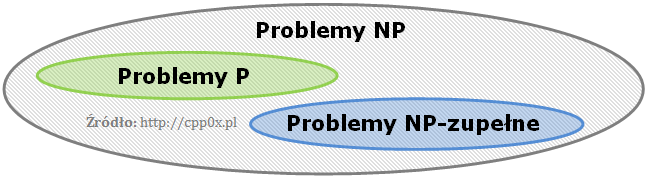
\includegraphics[width=0.6\textwidth]{k5_zbior_problemow_np.png}
\caption{Klasy złożoności}
\end{figure}

Aby określić złożoność stosowane są metody \textbf{oceny złożoności}. W celu ujednolicenia wyników i uniezależnienia się od środowiska, ocena złożoności rozpatrywana jest modelem abstrakcyjnym nie uwzględniającym platformy czy mocy obliczeniowej maszyny. Wyróżniamy następne modele złożoności:
\begin{enumerate}
	\item \textbf{Czasowe} - czas wykonywania algorytmu wynikająca z liczby operacji elementarnych wykonywanych podczas przebiegu programu.
	\item \textbf{Pamięciowe} - pamięcio-żerność oraz zasobo-żerność - ilość pamięci operacyjnej, bądź przestrzeni dyskowej potrzebnej do rozwiązania problemu. Zależy od liczby oraz złożoności użytych struktur.
\end{enumerate}

Przy wyborze algorytmu zazwyczaj decydująca jest złożoność czasowa - o wiele bardziej miarodajny model.

Wyróżniamy także podział złożoności algorytmów ze względu na instancję problemu:
\begin{enumerate}
	\item \textbf{Optymistyczna} - najlepszy możliwy przypadek (minimalna ilość wykonywanych operacji).
	\item \textbf{Pesymistyczna} - najgorszy scenariusz (wykonywane są wszystkie operacje).
	\item \textbf{Średnia} - wartość oczekiwana wykonywania algorytmu.
\end{enumerate}

Do oceny złożoności algorytmu potrzebny jest \textbf{rząd wielkości} oraz zmienność zależnie od instancji problemu. Nie potrzebne są dokładne wartości, dlatego też stosuje się \textbf{asymptotyczne tempo wzrostu}, które to informuje nas o zmianie (wzroście bądź spadku) złożoności algorytmu w zależności od ilości danych wejściowych. Opisuje jak szybko funkcja rośnie, maleje, bądź pozostaje stała.

Asymptotyczne tempo wzrostu określane jest za pomocą \textit{notacji asymptotycznych}. Istnieje kilka notacji \textit{Bachmann-Landaua}:
\begin{itemize}
	\item $\mathcal{O}$ (omikron, duże O)  - Funkcja asymptotycznie \textbf{niewiększa}. Jest to ograniczenie górne, czyli taka funkcja, dla której wszystkie wartości funkcji badanej, będą od niej niewiększe (mniejsze bądź równe).
	\item $\Omega$ (omega) - Funkcja asymptotycznie \textbf{niemniejsza}. Jest to granica dolna, czyli funkcja, dla której wszystkie wartości funkcji badanej, będą od niej niemniejsze (większe bądź równe).
	\item $\Theta$ (theta) - Funkcja asymptotycznie \textbf{podobna}. Jest to oszacowanie dokładne, czyli funkcje ograniczające badaną funkcję od góry i od dołu.
	\item $o$ - (małe O) - Funkcja asymptotycznie mniejsza. Rzadko stosowana.
	\item $\omega$ - (mała omega) - Funkcja asymptotycznie większa. Rzadko stosowana.
\end{itemize}

Złożoności kategoryzuje się do rzędów złożoności. Określają one jak szybko złożoność algorytmu rośnie wzraz ze wzrostem instancji problemu.

\begin{figure}[!h]
\centering
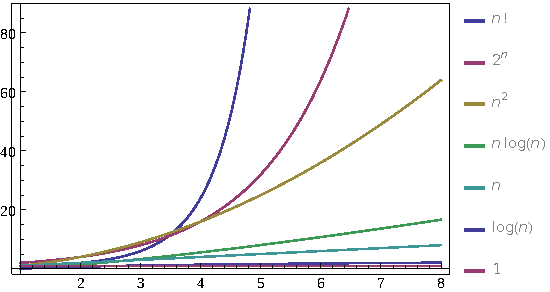
\includegraphics[width=0.8\textwidth]{k5_wykres_wszystkie.pdf}
\caption{Porównanie rzędów złożoności}
\end{figure}

Wyróżnić można (\textit{n - liczba danych wejściowych}):
\begin{itemize}
	\item $\mathcal{O}(1)$ - \textbf{złożoność stała} -  liczba operacji jest niezależna od rozmiaru problemu. Przykład: Ustalenie, czy liczba binarna jest dodatnia bądź ujemna, obliczenie $(-1)^n$, odwołanie się do n-tego elementu stałej w rozmiarze tablicy.
	\item $\mathcal{O}(\log n)$ - \textbf{logarytmiczna} - liczba operacji rośnie proporcjonalnie do logarytmu z rozmiaru problemu. Przykład: Wyszukiwanie binarne w posortowanej tablicy, dodanie/usunięcie elementu z drzewa binarnego.
	\item $\mathcal{O}(n)$ - \textbf{liniowa} - liczba operacji jest wprost proporcjonalna do rozmiaru problemu. Przykład: Znalezienie min/max elementu w nieposortowanej tablicy, dodanie dwóch n-bitowych liczb całkowitych w sumatorze z przeniesieniem szeregowym.
	\item $\mathcal{O}(n\log n)$ - \textbf{quasi-liniowa} - liczba operacji proporcjonalna do iloczynu rozmiaru problemu i jego logarytmu. Sortowania przez porównania (MergeSort (przez scalenie), HeapSort (kopcowe), QuickSort (szybkie)), FFT (Szybka Transformata Fouriera).
	\item $\mathcal{O}(n^2)$ - \textbf{kwadratowa} - liczba operacji rośnie proporcjonalnie do kwadratu rozmiaru problemu. Przykład: Prosty algorytm mnożenia dwóch n-bitowych liczb, sortowania: BubbleSort (bąbelkowe), SelectionSort (przez wybieranie), InsertionSort (przez wstawianie), znalezienie najkrótszej ścieżki w grafie.
	\item $\mathcal{O}(n^k)$ - \textbf{wielomianowa} - liczba operacji rośnie proporcjonalnie do wielomianu rozmiaru problemu. Przykład: Programowanie liniowe, maksymalne skojarzenie dla grafu dwudzielnego.
	\item $\mathcal{O}(2^n)$ - \textbf{wykładnicza} - liczba operacji rośnie proporcjonalnie do wartości wykładniczej rozmiaru problemu. Przykład: Programowanie dynamiczne dla problemu komiwojażera.
	\item $\mathcal{O}(n!)$ - \textbf{rzędu silnia} - liczba operacji rośnie proporcjonalnie do silni rozmiaru problemu. Przykład: Algorytm brute-force dla problemu komiwojażera.
\end{itemize}

\clearpage
\section{K6 - Język UML w projektowaniu oprogramowania}

UML w kontekście projektowania oprogramowania jest językiem pozwalającym na modelowanie i opisywanie systemów i ich części.

Pozwala na standaryzowany, graficzny zapis systemu z uwzględnieniem zarówno jego części konceptualnych, takich jak funkcje i procesy biznesowe, jak i obiektów fizycznych jakimi mogą być bazy danych czy warstwa sprzętowa.

W jaki sposób używa się UMLa do modelowania? Korzysta się z diagramów, które są podzielone ze względu na modelowanie strukturalne -- diagramy pakietów, klas, komponentów itd -- oraz behawioralne -- diagramy sekwencji, przypadków użycia, stanu itd.

UML jest przydatnym narzędziem nie tylko w procesie modelowania, ale również podczas szybkich rozmów między programistami kiedy chce się szybko nakreślić ideę.

Omówmy kilka najczęściej spotykanych diagramów.

\subsection{Diagramy strukturalne}
\subsubsection{Diagram pakietów}
Pełni rolę organizacyjną. Zawiera w sobie inne elementy języka, zazwyczaj diagramy klas.

\subsubsection{Diagram klas}
Składa się z zamodelowanych klas oraz relacji między nimi.

Pojedynczą klasę umieszcza się w prostokącie podzielonym na trzy części
\begin{itemize}
	\item{nazwę,}
	\item{atrybuty,}
	\item{funkcje.}
\end{itemize}

Atrybuty oraz funkcje oznacza się modyfikatorem dostępu (np. + dla public, - dla private), składniki statyczne zaznacza się poprzez podkreślenie, a stereotypy -- elementy służące do doprecyzowania semantyki elementu, np. oznaczenie jako klucz główny -- umieszcza się w podwójnych nawiasach ostrych <<>>.

Relacje między klasami:
\begin{itemize}
	\item{\textbf{Zależność -- strzałka przerywana} -- podstawowa relacja mówiąca, że obiekt może w jakiś sposób korzystać lub wpływać na inne obiekty.}
	\item{\textbf{Asocjacja -- linia ciągła} -- obiekty wykorzystują inne obiekty (człowiek używa magazynu do przechowywania rzeczy).}
	\item{\textbf{Agregacja częściowa -- pusta strzałka z rombem} -- obiekt posiada inne obiekty, ale nie są one do niego przypisane na wyłączność (kiedy człowiek umrze, jego samochód dalej istnieje).}
	\item{\textbf{Agregacja całkowita -- pełna strzałka z rombem} -- obiekt posiada inne obiekty i jest za nie odpowiedzialny (kiedy człowiek umrze, jego serce umiera wraz z nim).}
	\item{\textbf{Dziedziczenie --} pusta strzałka -- określa hierarchię dziedziczenia.}
\end{itemize}

\subsection{Diagramy behawioralne}
\subsubsection{Diagram przypadków użycia}
Diagram umożliwia analizę oraz dokumentację wymagań co do funkcjonalności systemu -- w jasny sposób pokazuje co jest od niego wymagane i pomaga w opracowaniu projektu oraz przetestowaniu już zbudowanego systemu. Co ważne, diagram nie posiada szczegółowych informacji na temat przypadków użycia -- takie informacje są umieszczane np. na diagramie stanu czy aktywności.

Diagram składa się z
\begin{itemize}
	\item{przypadków użycia -- ciąg akcji, z uwzględnieniem ich różnych wariantów, które mogą zostać wykonane podczas interakcji systemu z użytkownikiem,}
	\item{aktorów -- mogą być to ludzie-użytkownicy, ale również inne systemy czy urządzenia,}
	\item{związków -- powiązanie pomiędzy elementami diagramu.}
\end{itemize}
\subsubsection{Diagram sekwencji}
Pokazuje w sposób zgodny z intuicją kolejność wywołanych operacji i przepływ sterowania pomiędzy obiektami.

Diagram zbudowany jest z
\begin{itemize}
	\item{prostokątów, które oznaczają obiekty,}
	\item{pionowych linii życia tychże obiektów,}
	\item{komunikatów wymienianych między obiektami.}
\end{itemize}

Czas jest reprezentowany w postaci pionowej osi diagramu, a zajętość obiektu jest symbolizowana przez prostokąt umieszczony na jego linii życia.

Do komunikatów wymienianych między obiektami zalicza się między innymi
\begin{itemize}
	\item{wywołanie funkcji,}
	\item{powrót z wywołania,}
	\item{wywołanie asynchroniczne.}
\end{itemize}






\clearpage
\section{Generowanie realistycznych obrazów scen 3-D za pomocą metody śledzenia promieni}

\textbf{Fotorealizm} jest to metodyka starająca się w jak najlepszym stopniu oddać świat rzeczywisty za pomocą wygenerowanego obrazu. Aby to osiągnąć wykorzystuje się różne metody takie jak \textit{fotogrametria} (łączenie zdjęć tego samego obiektu z wielu różnych perspektyw w celu wygenerowania obiektu 3-D - technologia użyta np. przy tworzeniu gry \textit{The Vanishing of Ethan Carter}), metody próbkowania przestrzeni, czy też metoda śledzenia promieni. 

\textbf{Metoda próbkowania przestrzeni} polega na analizowaniu toru promieni od źródła światła, poprzez odbicia od obiektów sceny, aby finalne trafić do oka obserwatora albo wylecieć poza scenę. Z każdego źródła światła wyprowadzany jest pęk promieni (\textbf{dyskretyzacja światła}), i im więcej promieni, tym dokładniejszy stanie się obraz. Tutaj pojawia się problem, gdyż generowana jest bardzo duża liczba promieni, z czego ogromna większość nie przecina nawet rzutni (nie dociera do oka obserwatora), przez co operacje wykonane zostały bezsensownie. Stąd też wymyślona została metoda śledzenia promieni rozwiązująca ten problem.

\textbf{Metoda śledzenia promieni} (ang. \textit{Ray Tracing}) jest techniką służącą do generowania fotorealistycznych scen trójwymiarowych 3-D. Opiera się na śledzeniu wyłącznie tych promieni, które docierają do obserwatora. Cechą charakterystyczną jest to, że promienie nie są analizowane normalnym torem, tj. od źródła światła, bądź światła odbitego, do obserwatora, lecz właśnie \textbf{od oka obserwatora do elementów na scenie}. Zatem dla każdego piksela obrazu wynikowego wyprowadzany jest jeden promień, od którego w następstwie zależy wartość koloru tego piksela.

Wyprowadzony promień może nie trafić w żaden obiekt na scenie - piksel przyjmuje wtedy określony kolor tła. Promień może także trafić na źródło światła - piksel zyskuje kolor źródłowy światła. Promień może również trafić w jakiś obiekt na scenie. Jeśli trafi na taki obiekt, to wyznaczane są \textbf{punkty przecięcia}, następnie brany jest punkt najbliższy początkowi promienia i dla niego obliczany jest kolor punktu za pomocą wybranego modelu oświetlenia, na przykład popularnego \textbf{modelu Phonga}. Obliczane są w tym momencie także cienie używając pomocniczych promieni biegnących do źródła światła - gdy wiązka przetnie inny obiekt to oryginalny punkt jest zaciemniony. Całą procedurę można następnie powtarzać rekurencyjnie śledząc kolejne promienie odbite (zwane wtórnymi) i załamane tak, aby uzyskać efekt przedmiotów odbijających się w sobie nawzajem.

Przebieg działania algorytmu zapisywany jest w postaci \textbf{drzewa} (graf nieskierowany). Skrócony przebieg algorytmu przedstawić można w kilku krokach:
\begin{enumerate}
	\item Dla każdego piksela obrazu wyprowadź \textbf{promień pierwotny}.
    \item Dla każedgo napotkanego obiektu oblicz odbicia i wyprowadź \textbf{promienie wtóre}. Każdy punkt odbicia zapisz jako nowy węzeł drzewa.
    \item Dla każdego węzła wyznacz oświetlenie lokalne korzystając z wybranego modelu oświetlenia.
    \item Przechodząc od liści drzewa dodawaj kolejne wartości oświetlenia lokalnego ustalając tym samym ostateczną wartość piksela, od którego wyszedł promień pierwotny.
\end{enumerate}

Algorytm kończy swe działanie w momencie, gdy:
\begin{itemize}
	\item Promień nie trafia w żaden obiekt na scenie
    \item Promień trafia w obiekt całkowicie rozpraszający światło
    \item Promień trafia na obiekt, w którym następuje całkowite wewnętrzne odbicie
    \item Wyczerpana została ilość rekursywnych odbić
\end{itemize}

\textbf{Model Phonga} służy do wyznaczania oświetleń lokalnych. Na model ten składają się trzy rodzaje oświetlenia:
\begin{enumerate}
	\item \textbf{Światło ambientowe} - światło otoczenia, jest to wartość stała przypisana do danej sceny.
	\item \textbf{Światło rozproszone} - podstawowy kolor obiektu, wyliczany na podstawie \textbf{modelu Lamberta} (\textit{Lambert, Lambert ty chuju} - Wiedźmin Geralt z Rivii) i widoczny przede wszystkim na powierzchniach matowych (drewno, papier).
	\item \textbf{Światło odbite} - odpowiada za efekt połysku dla powierzchni śliskich, błyszczących (Passat metallic nówka nie śmigana trzy razy klepana). Wskazuje kierunek promienia odbitego.
\end{enumerate}

\begin{figure}[!h]
\centering
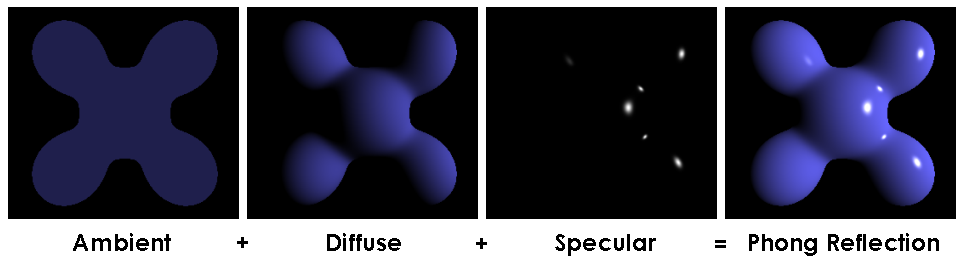
\includegraphics[width=0.8\textwidth]{k7_model_phonga.png}
\caption{Model Phonga}
\end{figure}

Owe składowe są mnożone przez procentowy współczynnik wpływu każdej składowej a następnie sumowane według poniższego wzoru:

\begin{equation}
I = k_{a}I_{a} + k_{d}I_{d} + k_{s}I_{s}
\end{equation}

Gdzie:
\begin{itemize}
	\item $I$ – natężenie światła w punkcie
	\item $I_{a}$ – (ang. \textit{ambient}) natężenie światła otoczenia
    \item $I_{d}$ – (ang. \textit{diffuse}) natężenie światła rozproszonego
    \item $I_{s}$ – (ang. \textit{specular}) natężenie światła odbitego lustrzanie
	\item $k$ – procentowy współczynnik wpływu składowych (przypisane do danego obiektu)
\end{itemize}

\textbf{Prawo Lamberta} mówi, że natężenie światła rozproszonego jest wprost proporcjonalne do kosinusa kąta pomiędzy wektorem promienia a wektorem normalnym do powierzchni. W skrócie - im mniejszy kąt, tym mniej światła jest rozproszone (powierzchnia skierowana prostopadle do promienia jest najjaśniejsza).

W modelu Phonga używany jest także dodatkowy efekt zway \textbf{tłumieniem atmosferycznym}, polegające na spadku natężenia światła wraz z rosnącą odległością od obserwatora. Zjawisko to można wykorzystać do generacji realistycznych warunków pogodowych, takich jak deszcz, zamieć, mgła.

Metoda śledzenia promieni mimo, że daje zdumiewające rezultaty to ma w sobie kilka poważnych wad:
\begin{itemize}
	\item Jest \textbf{bardzo kosztowna obliczeniowo} przez dużą liczbę obliczeń potrzebnych do wyliczenia koloru każdego piksela. Najbardziej kosztowne jest liczenie kolizji, co optymalizować można np. algorytmem brył otaczających, czyli wpisaniem zaawansowanych brył w większe, prostsze kształty - jeśli nie wystąpi kolizja z prostym kształtem, to na pewno nie nastąpi także z tym zaawansowanym.
    \item Może występować \textbf{zjawisko aliasingu}, które sprawia, że niektóre małe obiekty są pomijane, a obiekty o ostrych krawędziach mogą być zniekształcone (poszarpane). W celu uniknięcia tego problemu stosowanych jest wiele metod \textbf{antyaliasingu} na przykład nadpróbkowanie (\textit{supersampling - SSAA}), gdzie jeden promień pierwotny zastępowany jest \textbf{wiązką promieni} i kolor piksela jest zazwyczaj średnią z tej wiązki
    \item Przyrost ilości źródeł światła i obiektów znacznie pogorsza czas renderowania
    \item Nie wszystkie kierunki padania promieni są rozpatrywane
    \item Każdą klatkę trzeba generować od nowa - nie można wykorzystać informacji z poprzednich klatek
\end{itemize}

Wartym zaznaczenia jest fakt, że \textbf{śledzenie promieni dla każdego z pikseli odbywa się niezależnie} od innych pikseli, także metodę tę można \textbf{zrównoleglić} (zarówno dla grupy pikseli bądź promieni) na przykład wykorzystując zestawy instrukcji MMX oraz SSE z architektury SIMD równoleglące te same operacje arytmetyczne na liczbach całkowitych w procesorze, bądź używając do tego celu dobrodziejstw najnowszych procesorów graficznych - na przykład technologii NVIDIA CUDA, która pozwala na otrzymanie obrazu generowanego tą metodą w czasie rzeczywistym.
\clearpage
\sloppy\section{K8 -- Mechanizmy systemu operacyjnego wspomagające synchronizację procesów.}

Zarządzanie procesami to ważne zadanie systemu operacyjnego. \textbf{Program} to statyczny obiekt, zbiór instrukcji dla procesora, przechowywany w postaci pliku. \textbf{Proces} natomiast to wykonujący się program. Każdy proces wymaga przydziału zasobów (czas procesora, pamięć, pliki) do wykonania swojego zadania. Obsługa procesów jest wykonywana przez jądro systemu operacyjnego.

Problem synchronizacji procesów pojawia się przy procesach współbieżnych, które ze sobą współpracują. Przykłady, w których wymagana jest synchronizacja procesów to:
\begin{itemize}
\item problem sekcji krytycznej -- procesy współdzielą strukturę danych, a operacje na nich muszą być atomowe,
\item problem czytelników i pisarzy -- synchronizacja dostępu do zasobów dla procesów dokonujących i niedokonujących w nich zmian,
\item problem producenta i konsumenta -- wynik działania jednego procesu wpływa na działanie drugiego procesu -- przetwarzanie danych przez drugi proces może się odbyć jedynie, gdy zostanie dane zostaną przekazane przez pierwszy proces,
\item problem ucztujących filozofów -- procesy korzystają ze wspólnych zasobów, które pobierają i zwalniają wg potrzeb.
\end{itemize}

\textbf{Sekcja krytyczna} to sekwencja operacji wykonywanych na zasobie (np. pamięci, pliku), który musi być wykonywany w trybie wyłącznym przez jeden proces. Poprawnym rozwiązaniem sekcji krytycznej jest:
\begin{itemize}
\item instrukcje w sekcji krytycznej nie mogą być przeplatane -- może w niej być wyłącznie jeden proces,
\item nie można zakładać w jakiej kolejności i z jaką szybkością wykonają się dane procesy,
\item proces nie może zatrzymać się w sekcji krytycznej,
\item nie mogą występować zakleszczenia (jeden proces czeka na zwolnienie zasobów przez drugi, a drugi czeka na zwolnienie zasobów pierwszego, więc obydwa się zatrzymują),
\item każdy proces musi wejść do sekcji krytycznej (nie może wystąpić zagłodzenie).
\end{itemize}

Istnieją przeróżne mechanizmy synchronizacji implementowane przez jądro.

\textbf{Semafory} są typem danych, które służą do kontroli dostępu zasobów przez wiele procesów. Semafory są zmienną całkowitą, która przyjmuje wartości nieujemne (tj. $\ge 0$) lub dla semaforów binarnych -- wartości logiczne. Semafor ma wartość początkową nieujemną. Na semaforach można wykonywać dwie operacje -- zmniejszenie (zajęcie, podniesienie,) oraz zwiększenie (zwolnienie, opuszczenie). Synchronizacja polega na blokowaniu procesu w operacji zajęcia semafora do czasu, aż wartość nie zostanie zwiększona (np. przez inny proces, który zwolni semafor). Wyróżnia się rodzaje semaforów takie jak:
\begin{itemize}
\item binarne -- zmienna przyjmuje tylko wartości \textit{true} (semafor otwarty) lub \textit{false} (semafor zamknięty),
\item zliczające -- zmienna przyjmuje wartości całkowite nieujemne, a aktualna wartość jest zwiększana/zmniejszana o 1 w wyniku zwolnienia/zajęcia semafora,
\item uogólniony -- semafor zliczający, ale może zwiększać/zmniejszać wartość o dowolną liczbę (oczywiście, aby wartość wciąż była nieujemna).
\end{itemize}

\textbf{Muteksy} (\texttt{\textbf{mut}ual \textbf{ex}clusion} -- wzajemne wykluczanie) są szczególnym przypadkiem semaforów. Muteks może być zablokowany lub odblokowany. Muteksy mogą być zwalniane tylko i wyłącznie przez proces, który zajął dany muteks. Dzięki temu wyeliminowane jest zjawisko zakleszczenia oraz niespójności danych.

\textbf{Spinlocki} -- podobne do semaforów, jednak oczekiwanie na zwolnienie blokady odbywa się na zasadzie aktywnego czekania, przez co zajmują czas procesora, może wystąpić zagłodzenie lub czekać w nieskończoność.

\textbf{Monitory} są strukturalnym narzędziem synchronizacji wątków. Składają się ze zmiennych oraz procedur operujących na nich, zebrane w jeden moduł. Dostęp do zmiennych jest możliwy wyłącznie za pomocą procedur monitora, a w danej chwili tylko jeden proces może wywoływać procedury monitora. Gdy inny proces wywoła procedurę monitora, to będzie on zablokowany do chwili opuszczenia monitora przez pierwszy proces. Istnieje możliwość wstrzymania i wznowienia procedur monitora za pomocą zmiennych warunkowych. Na zmiennych warunkowych można wykonywać operacje \texttt{wait} (wstrzymanie procesu i umieszczenie go na końcu kolejki) oraz \texttt{signal} (odblokowanie jednego z oczekujących procesów). Procesy oczekujące na wejście do monitora zorganizowane są w kolejkę FIFO.
\clearpage
\sloppy\section{K9 -- Programowalne scalone układy cyfrowe PLD, CPLD oraz FPGA}

Programowalne układy scalone to układy scalone, których funkcjonalność jest definiowana przez użytkownika końcowego, a nie producenta. Wszystkie wyprodukowane przez producenta układy są identyczne (co pozwala zmniejszyć koszty). Pozwala to na zaprojektowanie, uruchomienie i testowanie urządzenia. Programowanie odbywa się za pomocą tworzenia połączeń w istniejącej sieci ścieżek sygnałowych. 

Układy programowalne można podzielić ze względu na ich strukturę:
\begin{itemize}
\item PLD -- (programmable logic device) najprostsze,
\item CPLD -- complex PLD,
\item FPGA -- field-programmable gate array.
\end{itemize}

Układy PLD mogą realizować funkcje logiczne (tworząc układy kombinacyjne bądź sekwencyjne). Programowanie takich układów bazuje na ustawieniu odpowiednich bitów, by zostały zrealizowane dane funkcje. Każde urządzenie posiada dany zbiór wejść oraz wyjść do układu.

Najprostsze układy PLD (SPLD) pozwalają na tworzenie prostych układów. Do nich możemy zaliczyć układy PLE, PAL, PLA. Ich budowa opiera się na matrycach funkcji AND oraz OR -- realizują funkcje postaci $(x_{1} \wedge x_{2} \wedge ...) \vee (x_{m} \wedge x_{m+1} \wedge ...) \vee ...$ lub $(x_{1} \vee x_{2} \vee ...) \wedge (x_{m} \vee x_{m+1} \vee ...) \wedge ...$ (dla sklerotyków: $\wedge$ -- AND, $\vee$ -- OR). 

Układy PLA posiadają programowalne matryce AND oraz OR. Dowolna linia iloczynu logicznego z matrycy AND (tzw. \textit{term}) może zostać podłączony do realizacji dowolnej operacji sumy logicznej OR. Inna architektura, PAL posiada programowalną matrycę AND oraz stałą (nieprogramowalną) matrycę OR. Natomiast układy PLE posiadają stałą matrycę bramek AND oraz programowalną matrycę bramek OR.

Układy CPLD, jak nazwa wskazuje są bardziej złożone. Zbudowane są z zespołu struktur SPLD połączonych ze sobą programowalną matrycą (switching matrix). Blok funkcjonalny CPLD posiada matrycę AND, makrokomórki oraz zadaną liczbę wyjść. Makrokomórki składają się zazwyczaj z bramek (np. AND, OR) oraz przerzutników. Sygnały sterujące makrokomórkami można podzielić na globalne (wspólne dla wszystkich makrokomórek), lokalne (wspólne dla zespołu połączonych ze sobą makrokomórek) oraz indywidualne (wpływają na działanie jednej makrokomórki). Pojedyncza makrokomórka realizuje prostą funkcję logiczną, większa ich liczba może być połączona ze sobą w bloki funkcyjne, tworząc funkcje z większą liczbą zmiennych. 

Najbardziej skomplikowane są układy FPGA. Zbudowane są one z konfigurowalnych elementów logicznych (CLB). W skład elementu logicznego wchodzą zazwyczaj generator funkcji logicznych, przerzutnik i programowalne multipleksery. Generator funkcji logicznych określany jest jako LUT (look up table). Elementy logiczne są łączone w bloki elementów logicznych. Połączenia między CLB są programowalne, podobnie jak w układach CPLD za pomocą programowalnej matrycy.

Do zalet struktur FPGA można zaliczyć elastyczność architektury (równoległość przetwarzania, dowolną szerokość ścieżki danych), wielokrotne użycie tych samych zasobów sprzętowych, czy też rekonfigurowalność.

Do programowania programowalnych układów scalonych wykorzystywane są języki opisu sprzętu, takie jak VHDL lub Verilog. Opis układu jest tworzony w sposób behawioralny. Narzędzie syntezy przetwarza taki zapis na konkretną realizację sprzętową. W porównaniu do układów ASIC (Full-Custom, Semi-Custom), takie układy są od nich szybsze. W przeciwieństwie do mikrokontrolerów, układy potrafią przetwarzać równolegle, a $\mu$C przetwarzają sekwencyjnie. Nie są one ograniczone zbiorem funkcji -- $\mu$C posiadają określony zestaw instrukcji. Wadą układów programowalnych w stosunku do nieprogramowalnych jest większy pobór mocy. Na układach programowalnych można zaprogramować procesor programowy -- PicoBlaze, MicroBlaze.

Układy PLD mają szerokie spektrum zastosowań. Można do tego zaliczyć logikę scalającą -- interfejs dla mikrokontrolerów umożliwiający współpracę z innymi modułami (pamięć, układy peryferyjne). Poprzez możliwość przetwarzania równoległego, układy PLD nadają się jako akceleratory sprzętowe. Akceleratory są wykorzystywane przy przetwarzaniu grafiki, dźwięku lub wideo.
\clearpage
\sloppy\section{K10 -- Optyczne nośniki informacji}

Dyski optyczne zaliczają się do nośników informacji. Zostały wprowadzone jako alternatywa dla dysków magnetycznych. Odczyt danych z dysku optycznego odbywa się za pomocą wiązki światła (a konkretniej promienia lasera) -- nazwa opiera się na zasadzie działania takiego nośnika.

W dzisiejszych czasach nośniki optyczne mają różne pojemności, stosowane są w różnych dziedzinach (np. na nich dystrybuowana jest muzyka, czy też filmy). 

Do dysków optycznych zaliczamy:

\textbf{LaserDisc} -- analogowy dysk optyczny, który miał 30 cm średnicy, składał się z dwóch jednostronnych aluminiowych dysków pokrytych plastikiem. Na nośniku był zapisywany analogowy sygnał wideo oraz analogowy i/lub cyfrowy sygnał dźwiękowy. Posiadał formaty kodowania:
\begin{itemize}
\item CAV -- stała prędkość kątowa, dyski pracowały ze stałą prędkością kątową 1800rpm, z odczytem jednej klatki na obrót, pojemność wynosiła 30 min na stronę, CAV posiadała funkcje stop klatki, zmiany prędkości odtwarzania oraz cofanie,
\item CLV -- stała prędkość liniowa, nie posiada funkcji z CAV, przez zmniejszenie prędkości obrotowej zwiększyła się pojemność do 60 min obrazu lub dźwięku,
\item CAA (wariant CLV) -- stałe przyspieszenie kątowe, wynalezione by wyeliminować zjawisko wchodzenia jednego kanału na drugi z CLV, różnica między CAA a CLV polega na dopasowaniu kąta obrotu dysku, zamiast stopniowego liniowego zwalniania, dzięki CAA znacznie poprawiła się jakość obrazu na nośniku,
\end{itemize}

\textbf{CompactDisk} -- początkowo był stworzony tylko do przechowywania muzyki, później dodano możliwość przechowywania danych. Płyta CD ma średnicę 12 cm i może pomieścić do 80 min dźwięku lub 700 MB danych. Istnieje również format mini-CD, jednak jest on mniej popularny (do 24 min dźwięku, 210 MB pojemności; inny format -- ,,wizytówka'' CD -- do 6 min dźwięku, do 65 MB pojemności). Formaty CD:
\begin{itemize}
\item Audio-CD -- format to dwukanałowy 16-bitowy PCM, z próbkowaniem 44.1 kHz na kanał, dźwięk mono nie występuje w implementacji, zazwyczaj dźwięk mono jest przedstawiony jako dwa takie same kanały w stereo. CD-Text jest rozszerzeniem Audio-CD, zezwala na zachowanie informacji tekstowych (np. nazwa albumu, artysty, ścieżek).
\item Video-CD -- cyfrowy standard do przechowywania wideo na płytach CD. W porównaniu z kasetami VHS jakość wideo nie pogarsza się po każdym użyciu. Wykorzystywane rozdzielczości to 352x240 oraz 352x288.
\item CD-R -- płyta może zostać raz zapisana, posiada warstwę barwnika, który jest stapiany przy zapisywaniu,
\item CD-RW -- płyta do zapisu wielokrotnego, kasowanie danych odbywa się za pomocą lasera (następuje topnienie stopu, traci swoją strukturę polikrystaliczną).
\end{itemize}

\textbf{DVD} -- medium do przechowywania różnego typu danych, zazwyczaj do oprogramowania oraz filmów. Nośniki posiadają takie same wymiary jak płyty CD, jednak można na nich zapisać więcej danych. Zwiększenie danych jest możliwe dzięki zwiększeniu gęstości zapisu danych (użyto lasera o krótszej długości fali). Powstały również płyty dwustronne oraz dwuwarstwowe. Podobnie jak w przypadku płyt CD, istnieją tutaj płyty jednokrotnego oraz wielokrotnego zapisu. Płyty DVD również posiadają formaty Audio oraz Video. Płyty audio posiadają dużą możliwość konfiguracji kanałów, z różnym próbkowaniem (nawet do 24-bit, 192 kHz). W porównaniu do CD-Audio pozwala zapisać więcej dźwięku w lepszej jakości. Zapis wideo na płytach DVD-Video wykorzystuje kodek MPEG-2. Najczęściej stosowane rozdzielczości to 720x576 oraz 720x480. Następcą DVD jest HD DVD, który zawierał gęstszy zapis danych, jednakże został porzucony na rzecz płyt Blu-Ray (wykorzystują tę samą długość fali lasera).

Dostęp do drugiej warstwy możliwy jest przez przepuszczenie lasera przez pierwszą, częściowo przepuszczalną warstwę. Zmiana ścieżki może potrwać kilka sekund, przez co może spowodować chwilowe zatrzymanie pracy napędu.

\textbf{Blu-ray} jest kolejnym formatem dysków optycznych. Dyski posiadają 25 GB na warstwę, przy zapisie dwu-warstwowym daje to 50 GB. W 2008 roku przedstawiono szesnasto-warstwową płytę BD, o pojemności 400 GB. Istnieją również formaty trzy- i cztero-warstwowe płyt BD. Nazwa technologii wywodzi się od koloru wykorzystywanego lasera. 

\begin{figure}[H]
\caption{Porównanie formatów płyt. Źródło: Wikipedia}
\centering
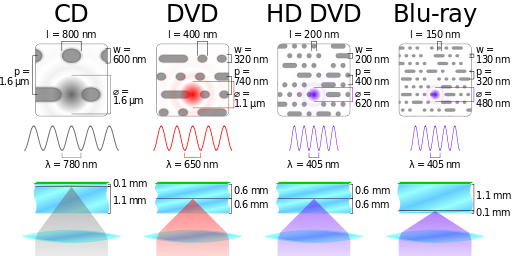
\includegraphics[width=\linewidth]{K10_Porownanie_plyt_Wikipedia.png}
\end{figure}

\textbf{HVD} (Holographic Versatile Disc) -- technologia dysków optycznej nowej generacji, teoretycznie pozwala pomieścić do 6 TB na jednej warstwie. Zapis danych odbywa się w trójwymiarowej przestrzeni dysku. Wykorzystywane są dwa lasery -- zielony oraz czerwony.

NRZI -- metoda odwzorowania sygnału binarnego, bez powrotów do zera. Wykorzystuje dwa stany logiczne. Przejście między nimi następuje, gdy transmitowany bit wynosi 1, w przypadku bitu 0 zmiana nie następuje.

Stany logiczne na płycie CD są reprezentowane przez pity (wgłębienia) oraz landy (płaskie powierzchnie, przerwy między wgłębieniami). Gdy wiązka trafia na pit, to jest rozpraszana i nie wraca do czytnika. Przy landzie wiązka jest odbijana i trafia z powrotem do czujnika. Każda przejście z landu na pit o odwrotnie powoduje zmianę stanu (logiczne 0 lub 1). Dane zapisywane są od środka na zewnątrz płyty.

\begin{figure}[H]
\caption{Stany logiczne odczytywane z powierzchni płyty}
\centering
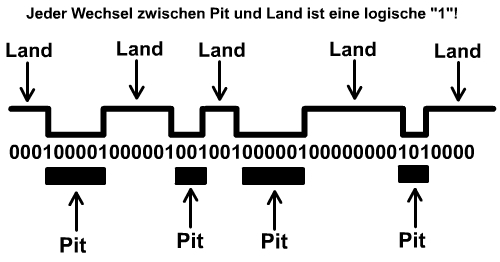
\includegraphics[width=\linewidth]{K10_pits.jpg}
\end{figure}

Kodowanie wykorzystywane w płytach to EFM (eight to fourteen modulation). Jest wykorzystywane ze względu na ograniczenia technologiczne (szybkości światła i odpowiedzi modulatora). Przez to długości pitów i landów muszą znajdować się w przedziale od 3 do 11 bitów kanałowych (ciąg kilku pitów/landów nie może być krótszy niż 3 bity kanałowe oraz dłuższy niż 11). Dlatego każde 8 bitów jest zapisywane za pomocą 14 bitów kanałowych. Do konwersji jest wykorzystywana tabela, która jest zapisana w firmware napędu. 

Dla płyt DVD, ze względu na mniejsze odległości stosowany jest zapis bajtów na 16 bitowych sekwencjach. Długości pitów i landów muszą być w przedziale od 3 do 14 bitów kanałowych.

Płyty Blu-ray wykorzystują kodowanie podobne do EFM, 17PP (one seven parity preserving). Wykorzystuje kodowanie, w którym każde 2 bity są zapisywane na 3 bitach, a samo kodowanie odbywa się w grupach po 2 albo 4 bity. Dodatkowo występują bity kontrolne (DC), po których wystąpieniu (jeśli DC == 1), zmieniana jest polaryzacja strumienia NRZI.

A teraz z innej beczki... Innym optycznym nośnikiem informacji są \textbf{kody kreskowe}. Skanery odczytują zapisane dane. Mogą być wydrukowane na różnych powierzchniach. Składają się z jasnych oraz ciemnych elementów. Istnieje wiele rodzajów kodów kreskowych, można je pogrupować według zastosowania, np. identyfikacja towarów (EAN, Code 11), kody pocztowe (POSTNET, PLANET, etc.). Istnieją również dwuwymiarowe kody kreskowe -- składają się one z macierzy elementów (jasnych/ciemnych). Do nich można zaliczyć kody takie jak: kody QR, czy Aztec Code (wykorzystywany w polskich dowodach rejestracyjnych).

Ten temat to temat rzeka, można opowiedzieć o wielu rzeczach (IrDA, światłowody i pewnie wiele innych). Ostatnim rodzajem, o którym chcę wspomnieć to dyski magnetooptyczne. Są stworzone z tworzywa sztucznego oraz warstwy materiału magnetycznego, zabezpieczone w kasecie, chroniąc przed uszkodzeniami mechanicznymi. Podobnie jak w wypadku płyt omówionych wcześniej, istnieją dyski magnetooptyczne zapisywane jedno- oraz wielokrotnie. Odczyt danych z takiego dysku wykorzystywane jest zjawisko Kerra (zmiana współczynnika załamania światła przez pole magnetyczne). Przy odbiciu lasera od namagnesowanego miejsca następuje ,,skręcenie'' w kierunku zależnym od pola magnetycznego i ta zmiana jest wykrywana przez głowicę napędu i traktowana jako stan logiczny.
\clearpage

\part{Pytania specjalnościowe -- INT}
\section{S1 - Tryby komunikacji między procesami w standardzie Message Passing Interface}

\clearpage
\section{S2 -- HTML DOM i XHTML -- cel i charakterystyka}

\subsection{HTML -- HyperTextMarkup Language}

\textbf{Cel:}
\begin{itemize}
\item Zapewnienie uniwersalnego, przenośnego, niezależnego od platformy sprzętowej i systemu operacyjnego standardu opisującego struktury strony internetowej;
\item Nadanie elementom strony odpowiedniego znaczenia semantycznego strony w zależności od ich zawartości np. tag \texttt{<em>};
\item Umożliwienie pozycjonowania strony w wyszukiwarkach internetowych w zależności od zawartości strony np. tag \texttt{<article>}
\end{itemize}

\textbf{Charakterystyka:}

Mianem HTML określamy standard języka znaczników używanego do tworzenia stron internetowych. Znaczniki są interpretowane przez przeglądarkę internetową i na ich podstawie w połączeniu ze stylami CSS oraz skryptami najczęściej napisanymi w języku JavaScript renderowana jest strona internetowa. Język jest niezależny od platformy sprzętowej oraz systemu operacyjnego, natomiast wymaga posiadania przeglądarki internetowej wspierającej standard w, którym napisano stronę. Znaczniki są słowami kluczowymi otoczonymi nawiasami ostrokątnymi. Zazwyczaj występują parami tzn. Istnieje tag otwierający i zamykający np.

\begin{verbatim}<p>This is some text in a paragraph.</p>\end{verbatim}

Tag zamykający zawiera / po otwarciu < . Występują, także tagi nie wymagające zamknięcia np. 

\begin{verbatim}<img src="smiley.gif" alt="Smiley face" height="42" width="42">\end{verbatim}

Tagi mogą posiadać atrybuty np. src w przykładzie wyżej. Atrybuty dzielą się na obowiązkowe i nieobowiązkowe. Atrybut obowiązkowy jest wymagany do prawidłowego działania danego tagu. Przykładowo, jeżeli nie podamy atrybutu src tagowi img nasz obraz nie wyświetli się. Natomiast atrybuty nieobowiązkowe nie są wymagane do prawidłowego działania tagu np. kiedy nie podamy atrybutu height zostanie on zastąpiony wartością domyślną. Często atrybuty zastępowane są wartościami ustawianymi dla danego tagu w języku CSS. Przyjmuje się konwencje, że nazwy znaczników pisane są małymi literami. Co ciekawe jeżeli spojrzymy na pierwszą stronę napisaną w tym języku były one pisane wielkimi literami.

HTML nie jest językiem restrykcyjnym. Kiedy projektant strony zapomni o zamknięciu jakiegoś tagu wówczas strona wyświetli się w przeglądarce, nie zostanie wyświetlony żaden błąd, a strona prawdopodobnie zostanie wyświetlona poprawnie zgodnie z oczekiwaniami. Oczywiście w przypadku nieprawidłowego kodowania dokumentu html wyświetlanie strony zależy od silnika danej przeglądarki. Obecnym standardem języka jest wersja 5 opublikowana oficjalnie w 2014 roku przez firmę W3C zajmującą się standaryzacją tego języka. W historii standaryzacją zajmowały się IETF oraz ISO. O standardzie strony informuje nas nagłówek zawarty w pierwszej linii pliku z rozszerzeniem .html. Najnowszy standard oznaczony jest jako \texttt{<!DOCTYPE html>}

W przypadku standardów zachowano kompatybilność wsteczną.

HTML 5 wprowadził wiele nowości w porównaniu do wersji 4 opublikowanej w 1997 roku. Są nimi nowe tagi np. \texttt{<article>}, \texttt{<aside>} mające w lepszy niż sposób niż dotychczas opisywać semantykę strony. Atrybuty możemy podawać otoczne nawiasami " " oraz ' ', a także bez nawiasów. Dodano tagi związane z przesyłaniem mediów jak <video> oraz <audio> niewymagające korzystania z dodatkowych bibliotek i wtyczek jak Silverlight lub Flash. Dodaje także funkcjonalności niezwiązne z tagami jak:
\begin{itemize}
\item Local storage \url{http://www.w3schools.com/html/html5_webstorage.asp}
\item Workery działające w tle \url{http://www.w3schools.com/html/html5_webworkers.asp}
\end{itemize}

Typowa struktura znaczników strony HTML:

\begin{figure}[H]
\centering
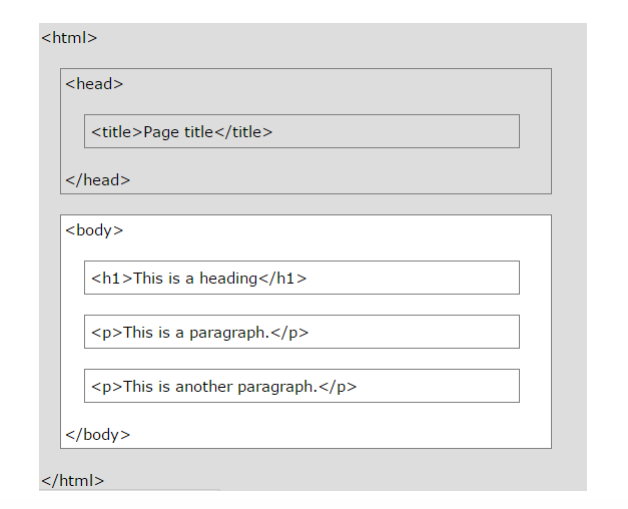
\includegraphics[width=0.6\linewidth]{s2_int_struktura.png}
\end{figure}

Stronę otacza tag \texttt{html} w nim zawarte są dwa podstawowe tagi \texttt{head} i \texttt{body}. \texttt{Head} zawiera metadane dotyczące strony: język, kodowanie, tytuł. Często umieszcza się dam odwołania do plików ze stylami css i skryptami js. W tagu body zawarte są wszystkie tagi związane z zawartością strony.

\subsection{Drzewo DOM -- Document Object Model}

\textbf{Cel:}
\begin{itemize}
\item Dostarczenie prostej reprezentacji hierarchii znaczników strony HTML.
\item Dostarczenie modelu umożliwiającego programiście modyfikować, dodawać, usuwać elementy dokumentu .html korzystając z własności drzewa (jego przeszukiwania)
\end{itemize}

\textbf{Charakterystyka:}

Dokument HTML możemy przedstawić w postaci drzewa, które rozpoczyna się od tzw. Klasy dokument reprezentującej aktualną stronę Internetową. Zawiera m.in. dane o szerokości i wysokości okna. Do jej atrybutów programista ma dostęp z poziomu języka JavaScript. Obrazek mówi więcej niż tysiąc słów:

\begin{figure}[H]
\centering
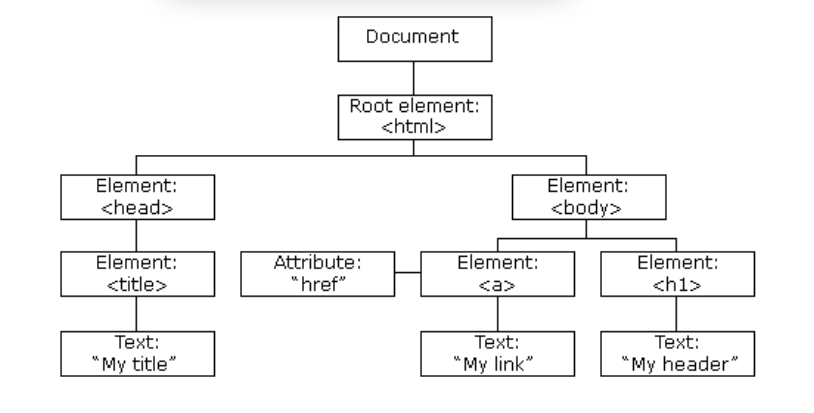
\includegraphics[width=0.9\linewidth]{s2_int_drzewo.png}
\end{figure}

Korzeniem jest tag \texttt{<html>}. Kolejne węzły stanowią tagi zawarte wewnątrz znacznika \texttt{<html>}. Dzieckiem węzła jest tag bezpośrednio zawarty wewnątrz danego tagu. 

\subsection{XHTML -- extensible Hyper Text Markup Language}

\textbf{Cel:}

Dostarczenie restrykcyjnego standardu rozszerzającego HTML, aby zwiększyć jakość stron internetowych wymagając od programistów poprawnej składni zgodnie z obowiązującym standardem.

\textbf{Charakterystyka:}

Jak już zostało wcześniej wspomniane w języku HTML, gdy programista popełni błąd strona zostanie wyświetlona przez przeglądarkę. Aby, zapewnić poprawność i spójność kodu został stworzony język XHTML. Posiada identyczne tagi i składnię jak w przypadku języka HTML. Jednak tutaj można wymienić kilka istotnych różnic:

\begin{itemize}
\item Jeśli strona XHTML zawiera błędy, nie może zostać wyświetlona;
\item Strony XHTML: \url{http://www.w3.org/1999/xhtml};
\item Element główny (html) musi zawierać atrybut xmlns określający przestrzeń nazw XHTML: \url{http://www.w3.org/1999/xhtml};
\item Znacznikowi otwierającemu każdego niepustego elementu powinien odpowiadać znacznik zamykający (np. \texttt{<li> ... </li>});
\item Puste elementy muszą także być zamykane (np. zamiast \texttt{<br>} musi być \texttt{<br/>}, albo \texttt{<br></br>});
\item Elementy muszą być zagnieżdżone w odpowiedni sposób (np. zamiast \texttt{<p>Tekst z <em>wyróżnieniem</p></em>} -- \texttt{<p>Tekst z <em>wyróżnieniem</em></p>}); wprawdzie w HTML także istniał taki wymóg, lecz nie był egzekwowany przez przeglądarki;
\item Nazwy elementów i atrybutów XHTML muszą być pisane małymi literami;
\item Wszystkie wartości atrybutów muszą być ujęte w cudzysłów (podwójny, np. \texttt{<td rowspan="3">}, albo apostrof, np. \texttt{<td rowspan='3'>});
\item Niedozwolona jest minimalizacja atrybutów (np. zamiast \texttt{<textarea readonly>} musi być \texttt{<textarea readonly="readonly">});
\item XHTML muszą mieć typ zawartości \texttt{application/xhtml+xml} (lub inny XML)
\end{itemize}

\clearpage
\section{S3 -- Asynchroniczna komunikacja serwerem HTTP w technologii AJAX}

Nazwa AJAX (Asynchronous JavaScript and XML) została wymyślona w 2005 roku. Miała ona opisywać istotę nowych narzędzi udostępnionych przez firmę Google (Google Suggest i Google Maps). Nie jest to oficjalna technologia tzn. nie ma na to standardu opisanego w RFC lub innym tego typu dokumencie. Określenie AJAX opisuje współdziałanie kilku technologii – języka JavaScript, protokołu http, mechanizmów przeglądarek internetowych i serwerów sieciowych. Generalnie AJAX mówi o asynchronicznej komunikacji z serwerem http, zapewniając pobieranie i wyświetlanie materiałów bez konieczności przeładowywania całej strony. Sama nazwa może być myląca, nie trzeba rozumieć XML, aby zrozumieć AJAX.

\textbf{Czym różni się komunikacja asynchroniczna od komunikacji synchronicznej?}

Komunikacja synchroniczna, to standardowy sposób komunikacji, kiedy to wysyłając zadanie blokując czekamy ze zwróceniem interfejsu do klienta, aż zadanie zostanie przetworzone. W przypadku krótkich transakcji taka sytuacja jest do przyjęcia, jednak w przypadku bardzo długich transakcji nie ma ona racji bytu. 
\begin{figure}[H]
\centering
\caption{Komunikacja synchroniczna}
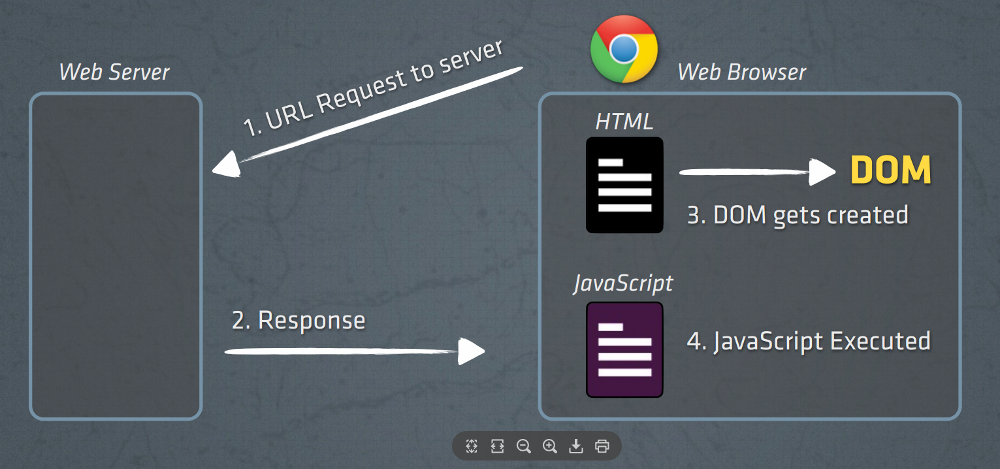
\includegraphics[width=\linewidth]{s3_int_kom_synchr.png}
\end{figure}

Komunikacja asynchroniczna pozwala nam wysyłać zapytanie w tle bez konieczność czekania ze zwróceniem interfejsu klienta. Kiedy zapytanie się skończy zostanie wywołana wcześniej zdefiniowana funkcja. Dzięki temu możemy:
\begin{itemize}
\item aktualizować zawartość strony przez konieczności przeładowywania całego drzewa DOM. 
\item wysyłać dane do serwera po załadowaniu się całej strony;
\item otrzymywać odpowiedź od serwera po załadowaniu się całej strony;
\item wysyłać dane do serwera w tle
\end{itemize}

\begin{figure}[H]
\centering
\caption{Komunikacja asynchroniczna}
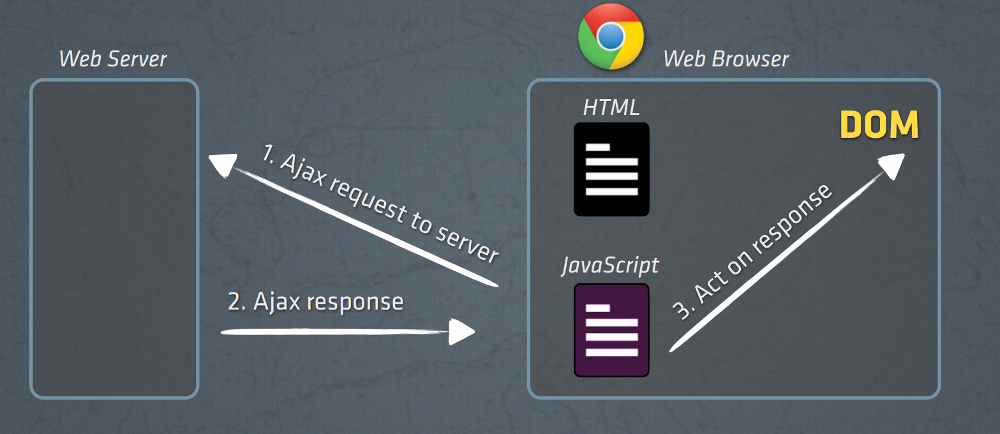
\includegraphics[width=\linewidth]{s3_int_kom_asynchr.png}
\end{figure}

Przykłady zastosowań AJAX:
\begin{itemize}
\item Wyświetlanie nowych danych HTML bez konieczności odświeżania strony;
\item Przesyłanie formularzy i natychmiastowe wyświetlanie wyników;
\item Logowanie bez opuszczania strony;
\item Kontrolka do oceny materiałów za pomocą liczby gwiazdek;
\item Przeglądanie informacji z bazy danych.  
\end{itemize}

Co jest nam potrzebne do rozpoczęcia działania? 
\begin{itemize}
\item \textbf{Przeglądarka internetowa} -- wbudowany obiekt XMLHttpRequest -- wprowadzony w przeglądarce Internet Explorer 5;
\item \textbf{Język JavaScript} -- wykonywanie zadań w AJAX-ie np. wysyła żądania na serwer, oczekuje i przetwarza odpowiedź, aktualizuje stronę przez dodanie nowych materiałów lub zmianę jej wyglądu
\item \textbf{Serwer Sieciowy} -- odbiera zadanie od przeglądarki i przesyła odpowiedź z danymi.
\end{itemize}
\begin{figure}[H]
\centering
\caption{Klasyczne AJAX-owe przetwarzanie}
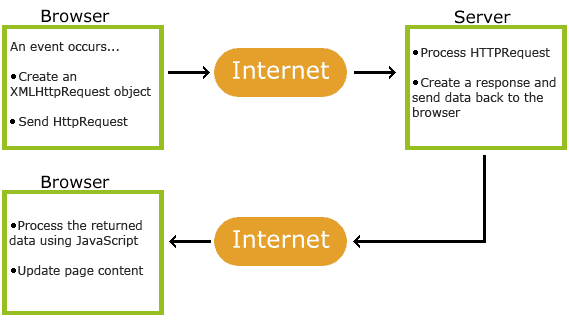
\includegraphics[width=0.8\linewidth]{s3_int_ajax_przetwarzanie.png}
\end{figure}

Implementacja zapytań ASYNCHRONICZNYCH w czystym JavaScripcie:
\begin{enumerate}
\item Utworzenie obiektu XMLHttpRequest (dostępny natywnie w przeglądarkach) -- więcej informacji \url{https://developer.mozilla.org/pl/docs/XMLHttpRequest}
\item Specyfikacja typu zapytania -- funkcja \texttt{open(method, url, async)};
\item Specyfikacja zdarzenia \texttt{onreadystatechange}:
\begin{enumerate}
\item pole obiektu XMLHttpRequest przechowuje funkcję, która jest automatycznie wywoływana kiedy \texttt{readyState} zmienia się;
\item pole \texttt{readyState} przechowuje status żądania HTTP zmieniającego się od 0 --- 4
\begin{enumerate}
\item 0 -- zapytanie niezainicjalizowane;
\item 1 -- nawiązanie połączenia z serwerem;
\item 2 -- zapytanie zostało otrzymane;
\item 3 -- przetwarzanie zapytania;
\item 4 -- zapytanie przetworzone, odpowiedź otrzymana;
\end{enumerate}
\end{enumerate}
\item Wysłanie zapytania funkcja send:
\begin{enumerate}
\item \texttt{send()} -- wysyła zapytanie wykorzystując GET;
\item \texttt{send(string)} -- wysyła dane na serwer;
\end{enumerate}
\end{enumerate}

\textbf{Obiekty promise -- JavaScript}
Obiekt promise jest używany do zadań asynchronicznych i odroczonych w czasie. Reprezentuje operację, która nie została jeszcze zakończona, ale oczekuje na zakończenie w przyszłości. Obiekt może znajdować się w 3 stanach:
\begin{itemize}
\item \texttt{pending} -- początkowy stan obiektu promise;
\item \texttt{fulfilled} -- stan reprezentujący operację zakończoną powodzeniem;
\item \texttt{rejected} -- stan reprezentujący operację zakończoną niepowodzeniem;
\end{itemize}
Obiekty promise wykorzystują do zapytań asnychronicznch biblioteki i frameworki webowe np. jQuery oraz AngularJS.



\clearpage
\section{S4 -- Technologie platformy Java EE}

\clearpage
\section{S5 -- Komunikacja procesów przez pamięć dzieloną}

Komunikacja międzyprocesowa jest potrzebna do poprawnego funkcjonowania systemów wieloprocesorowych. Istnieje wiele metod komunikacji między nimi. Można do nich zaliczyć metody takie jak: pliki, łącza nienazwane oraz nazwane, kolejki, gniazda, \textbf{pamięć dzieloną} i inne, np. MPI. Każda z nich zawiera charakterystyczne cechy, ma swoje wady i zalety. 

W odróżnieniu od wątków, komunikacja między procesami jest trudniejsza w zrealizowaniu, ponieważ wątki dzielą zmienne globalne oraz przestrzeń adresową. Każdy proces posiada własny kontekst i przestrzeń adresową -- procesy nie mogą ingerować w pamięć innych procesów, ponieważ to mogłoby mieć katastrofalne skutki.

Jak już wspominałem, istnieje wiele sposobów komunikacji międzyprocesowej. Jedną z nich jest komunikacja przez pamięć dzieloną. Jeżeli ktoś nie wie dlaczego tak to podkreślam, to zapraszam do zajrzenia na tytuł pytania egzaminacyjnego. Jest to jedna z najszybszych form komunikacji, ponieważ przesył danych między procesami nie jest wymagany, jądro nie jest pośrednikiem w komunikacji. Operacje odbywają się poprzez odwołanie do innych segmentów pamięci (ale pamiętajmy, że w wirtualnej przestrzeni adresowej, procesy nie operują na fizycznych adresach). Aby uzyskać taki segment, należy go najpierw odwzorować, za pomocą funkcji dostępnej w danej bibliotece (POSIX, WinAPI, Boost, etc.).

Należy jednak pamiętać, że wykorzystanie pamięci dzielonej, jak to z współbieżnością bywa, niesie ze sobą wymóg synchronizacji dostępu tej pamięci między procesami, które na niej operują. Możliwe rozwiązania synchronizacyjne to semafory, muteksy, monitory, etc. (więcej w punkcie dot. synchronizacji danych).

Istnieje wiele architektur, których celem jest współbieżne przetwarzanie. Jednakże, komunikacja przez pamięć dzieloną może zostać wykorzystana na systemach jedno- lub wieloprocesorowych, ze wspólną pamięcią. Niezależnie od wykorzystanej biblioteki, schemat wykorzystania pamięci współdzielonej jest podobny:
\begin{itemize}
\item utworzenie segmentu,
\item ustalenie rozmiaru segmentu,
\item odwzorowanie segmentu w przestrzeni adresowej procesu,
\item operacje na segmencie,
\item wycofanie odwzorowania,
\item odłączenie segmentu (gdy licznik odwołań użycia segmentu spadnie do zera, segment jest usuwany).
\end{itemize}
Wymogiem jest wzajemne wykluczanie, ponieważ nie powinno dojść do sytuacji, w których procesy modyfikują ten sam fragment danych -- może to mieć niepożądane skutki.

Zarówno w systemach UNIXowych oraz Windows wykorzystanie pamięci dzielonej działa na podobnej zasadzie. Standard POSIX, wykorzystywany w systemach UNIXowych udostępnia dwa zestawy funkcji do operacji na pamięci współdzielonej -- POSIX oraz System V. Nie można ich ze sobą mieszać.
\begin{itemize}
\item \texttt{shm\_open()/\textit{shmget()$^\star$}} - utworzenie segmentu
\item \texttt{ftruncate()/\textit{shmget()$^\star$}} - ustalenie rozmiaru segmentu
\item \texttt{mmap()/\textit{shmat()$^\star$}} - pobranie adresu odwzorowania segmentu
\item \texttt{munmap()/\textit{shmdt()$^\star$}} - wycofanie odwzorowania segmentu
\item \texttt{shm\_unlink()/\textit{shmctl()$^\star$}} - odłączenie segmentu
\end{itemize}
\textit{$^\star \to$ wywodzą się z \texttt{System V}};
w zestawie funkcji POSIX w odróżnieniu od System V, odwoływanie się do segmentów pamięci dzielonej (funkcje do tworzenia, odłączania segmentów) może odbywać się przez nazwy, w drugim standardzie poprzez indeksy.

Pamięć dzielona pozwala na komunikację pomiędzy różnymi procesami w jednym systemie. Jest to najszybszy sposób komunikacji, ponieważ nie wykorzystuje jądra. Wadą tego rozwiązania jest konieczność stosowania technik, które zapewniają poprawność przetwarzania danych. Oprócz tego, rozwiązanie to nie sprawdzi się w systemach sieciowych.
\clearpage
\section{S6 -- Metody komunikacji międzyprocesowej w systemach lokalnych i rozproszonych}

\textbf{Komunikacja międzyprocesowa} -- (\textit{Inter-Process Communication} -- IPC) -- sposób komunikacji pomiędzy wieloma procesami systemu operacyjnego uruchomionego na maszynie lokalnej, bądź rozproszonej grupie autonomicznych maszyn połączonych w sieć. Techniki komunikacji możemy podzielić na:
\begin{itemize}
	\item Przekazywanie komunikatów
    \item Synchronizację
    \item Współdzielenie pamięci
    \item Wywoływanie procedur
\end{itemize}

Główne cechy systemu rozproszonego:
\begin{itemize}
	\item \textbf{Dzielenie zasobów} -- maszyny rozproszonego systemu mają możliwość współdzielenia urządzeń (np. drukarki, skanery), dzielenia plików oraz usług
    \item \textbf{Otwartość} -- podatność na rozszerzenia, możliwość rozbudowy systemu zarówno sprzętowo jak i programowo
    \item \textbf{Współbieżność} -- zdolność przetwarzania wielu zadań równocześnie
    \item \textbf{Skalowalność} -- zachowanie podobnej wydajności systemu przy zmienianiu skali systemu (np. dodawanie nowych maszyn, procesorów)
    \item \textbf{Tolerowanie awarii} -- zdolność do dalszego działania systemu mimo wystąpienia błędów w oprogramowaniu lub uszkodzeń fizycznych
    \item \textbf{Przezroczystość} -- cały system zachowuje się tak, jakbyśmy pracowali na jednej maszynie, nie zaś na wielu osobnych jednostkach połączonych w jeden system
\end{itemize}

\begin{table}[!ht]
\centering
\caption{Metody komunikacji międzyprocesowej}
\label{ipc}
\begin{tabular}{|l|l|c|c|}
\hline
\multicolumn{1}{|c|}{\textbf{Metoda komunikacji}} & \multicolumn{1}{c|}{\textbf{Systemy operacyjne}} & \textbf{Lokalne} & \textbf{Rozproszone} \\ \hline
Pliki & Większość systemów & tak & tak \\ \hline
Gniazdka & Większość systemów & tak & tak \\ \hline
Sygnały & POSIX & tak & nie \\ \hline
Kolejki komunikatów & POSIX, Windows & tak & nie \\ \hline
Łącza nienazwane & POSIX, Windows & tak & nie \\ \hline
Łacza nazwane & POSIX, Windows & tak & nie \\ \hline
Semafory & POSIX, Windows & tak & nie \\ \hline
Pamięć współdzielona & POSIX, Windows & tak & nie \\ \hline
Zmapowany plik & POSIX, Windows & tak & tak \\ \hline
\begin{tabular}[c]{@{}l@{}}Przekazywanie\\ komunikatów\end{tabular} & \begin{tabular}[c]{@{}l@{}}Systemy z MPI, RPC,\\ COBRA, Java RMI\end{tabular} & tak & tak \\ \hline
\end{tabular}
\end{table}

\subsection{Pliki}

Jest to najłatwiejszy sposób wymagający jedynie otwarcia pliku. Dla zachowania spójności danych tylko jeden proces może zapisywać do pliku w danym czasie, zaś czytać może nieograniczona ilość procesów. Występuje tutaj potrzeba zastosowania jakiegoś sposobu synchronizacji procesów zapisujących i informowania innych o zmianach. Komunikacja może odbywać się w obrębie jednego systemu operacyjnego, bądź też między różnymi systemami współdzielącymi przestrzeń dyskową.

Przykłady funkcji POSIX:
\begin{itemize}
	\item \texttt{fopen()} -- otwarcie pliku
    \item \texttt{fwrite()} -- zapis do pliku
    \item \texttt{fread()} -- odczyt z pliku
    \item \texttt{fclose()} -- zamknięcie pliku
\end{itemize}

\subsection{Gniazdka}

Umożliwiają komunikację dwukierunkową w systemach lokalnych i rozproszonych -- pozwalają na odbieranie i wysyłanie danych po obu stronach. W systemach UNIX gniazdko traktowane jest jak deskryptor otwartego pliku, więc można na nim używać funkcji jak do plików (\texttt{read()}, \texttt{write()}, \texttt{close()}). Oba punkty końcowe połączenia identyfikowane są za pomocą adresu IP oraz portu. Komunikacja przebiegać może bezpołączeniowo po protokole UDP za pomocą ciągu niezależnych pakietów (datagramów), bądź połączeniowo po TCP czyli przy pomocy strumienia danych.

Przykłady funkcji POSIX:
\begin{itemize}
	\item \texttt{socket()} -- utworzenie gniazdka
    \item \texttt{bind()} -- nadanie gniazdku adresu
    \item \texttt{connect()} -- połączenie się z serwerem TCP
    \item \texttt{accept()} -- połączenie się z klientem TCP
    \item \texttt{listen()} -- rejestracja gniazdka TCP
    \item \texttt{send()}, \texttt{recv()} -- wysłanie i odebranie wiadomości TCP
    \item \texttt{sendto()}, \texttt{recvfrom()} -- wysłanie i odebranie wiadomości UDP 
    \item \texttt{write()}, \texttt{read()} -- wysłanie i odebranie wiadomości TCP a także UDP po wykonaniu asocjacji gniazdka funkcją \texttt{connect()}
    \item \texttt{close()} -- zamknięcie gniazdka
\end{itemize}

\subsection{Sygnały}

Znane także jako przerwania programowe -- są to asynchroniczne powiadomienia wysyłane do innych procesów wymagające natychmiastowej reakcji ze strony procesu. Źródłem przerwań może być system operacyjny gdy nastąpi wydarzenie awaryjne, wykonanie odpowiednich funkcji w programie, bądź zabicie programu spod konsoli funkcją kill. Po otrzymaniu przerwania, system zaprzestaje wykonywania aktualnych instrukcji (przerwana może być każda nie-atomowa operacja) i rozpoczyna obsługę przerwania wykonując ustalone wcześniej funkcje przechwyconych przerwań, bądź domyślne funkcje obsługi przerwań. Przechwycony może być każdy sygnał z wyjątkiem SIGKILL oraz SIGSTOP. Sygnały obsługiwane sątylko przy przejściu między trybem jądra systemu a trybem użytkownika.

\begin{figure}[!h]
\centering
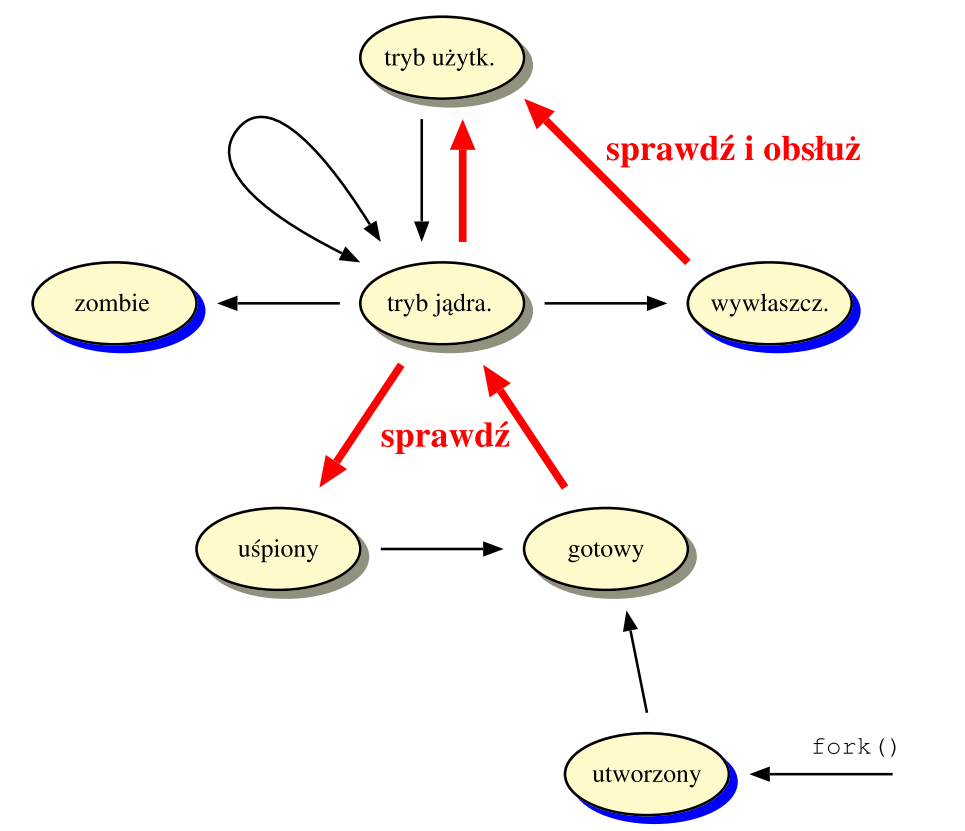
\includegraphics[width=0.6\textwidth]{s6_int_sygnaly.png}
\caption{Sygnały}
\end{figure}

Przykłady funkcji POSIX:
\begin{itemize}
	\item \texttt{signal()}, \texttt{sigset()} -- rejestruje funkcję obsługi sygnału
    \item \texttt{kill()}, \texttt{alarm()}, \texttt{raise()} -- wysyła sygnał
\end{itemize}

\subsection{Łącza nienazwane}

Jedna z prostszych metod komunikacji. Są to strumienie (pipe) pozwalające łączyć spokrewnione ze sobą procesy w relacji jednokierunkowej macierzysty -- potomny. Zazwyczaj są wykorzystywane do łączenia wyjścia stdout jednego procesu z wejściem stdin drugiego. Tworzenie łącza wypełnia dwuelementową tablicę deskryptorów, z czego pierwszy z nich jest końcem otwartym do czytania, a drugi służy do pisania. Oba końce traktowane są w systemie UNIX jako zwykłe deskryptory plików, więc można na nich używać funkcji jak do plików (\texttt{read()}, \texttt{write()}, \texttt{close()}). Nieużywany deskryptor musi zostać zamknięty funkcją \texttt{close()}. Jądro systemu gwarantuje, że operacje zapisu nie przekraczające rozmiaru bufora (w wielkości 4kB) są atomowe, niepodzielne. W powłokach systemów UNIX można używać łącza w formie pionowej linii do przesyłania wyników jednego polecenia do wejścia kolejnego.

\newpage

\begin{figure}[!h]
\centering
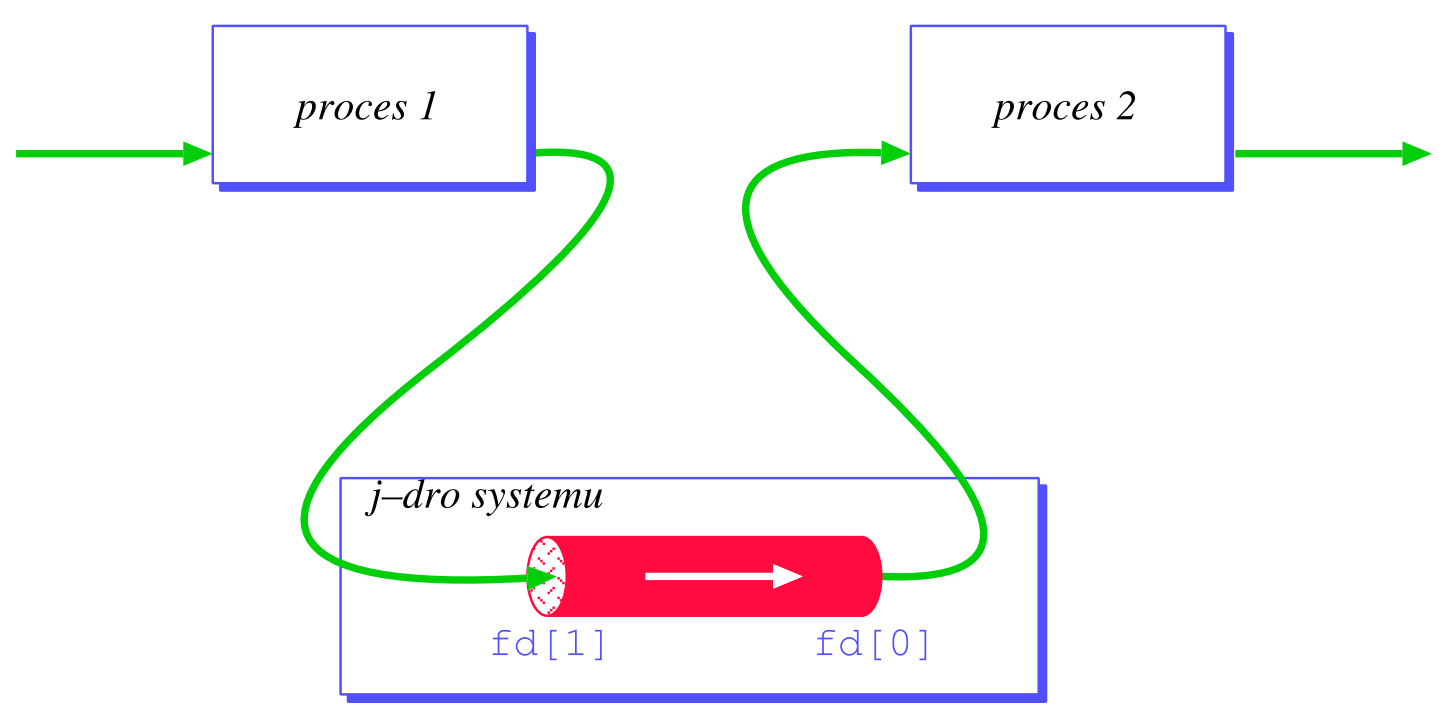
\includegraphics[width=0.8\textwidth]{s6_int_pipe.png}
\caption{Łącze nienazwane}
\end{figure}

Przykłady funkcji POSIX:
\begin{itemize}
	\item \texttt{pipe()} -- tworzy łącze nienazwane
    \item \texttt{dup()}, \texttt{dup2()} -- duplikowanie deskryptorów stdin, stdout
    \item \texttt{write()} -- zapisuje do łącza
    \item \texttt{read()} -- odczytuje z łącza
    \item \texttt{close()} -- zamyka łącze
\end{itemize}

\subsection{Łącza nazwane}

Inaczej strumienie FIFO, mogą być używane przez procesy w żaden sposób ze sobą nie spokrewnione, a nawet przez procesy różnych użytkowników. Szczególnie stosowane, gdy nie można zastosować relacji macierzysty -- potomny. Strumienie FIFO posiadają dowiązanie w systemie plików jako pliki specjalne -- oprócz atrybutów zwykłych plików takich jak nazwa, właściciel, grupa czy prawa dostępu, posiadają cechę dodatkową -- element odczytany z pliku FIFO jest z niego automatycznie usuwany. Funkcja użyta do otwarcia łącza blokuje proces do momentu otwarcia drugiego powiązanego łącza. Kolejki FIFO mają z reguły większy rozmiar 4-16kB.

Przykłady funkcji POSIX:
\begin{itemize}
	\item \texttt{mknod()} -- tworzy łącze nazwane
    \item \texttt{open()} -- otwiera łącze do pisania lub czytania
    \item \texttt{write()} -- zapisuje do łącza
    \item \texttt{read()} -- odczytuje z łącza
    \item \texttt{unlink()} -- usuwa łącze
\end{itemize}

\newpage

Miedzy łączami nienazwanymi a nazwanymi istnieje wiele podobieństw:
\begin{itemize}
	\item Zamknięcie końca do pisania generuje u czytelników EOF
    \item Zamknięcie końca do czytania generuje sygnał SIGPIPE u pisarzy
    \item Zapis i odczyt przez standardowe funkcje \texttt{read()} i \texttt{write()}
    \item Niepodzielność zapisu danych mniejszych niż rozmiar strumienia
    \item Blokowanie procesów w przypadku przepełnienia lub pustego bufora
\end{itemize}

\subsection{Kolejki komunikatów}

Jest to lista o określonej pojemności zawierająca komunikaty o zadanym maksymalnym rozmiarze. Komunikacja odbywa się tylko w jedną stronę -- nowe komunikaty dodawane są na koniec listy. Dzięki temu zachowana jest kolejność komunikatów. Każdy komunikat ma swój typ, dzięki czemu można obsługiwać kilka strumieni komunikatów w ramach jednej kolejki poprzez selektywne odbieranie komunikatów wybranego typu. Komunikacja odbywa się asynchronicznie, co znaczy, że odbiorca i nadawca nie muszą się łączyć w tym samym czasie. Komunikaty w kolejce ponadto przechowywane są do czasu odebrania ich przez inny proces. Kolejki komunikatów posiadają również inne ważne cechy:
\begin{itemize}
	\item Posiadają unikalne nazwy umożliwiające procesom identyfikację kolejki
    \item Można nadawać priorytety -- komunikaty o wyższym priorytecie są umieszczane na początku
    \item Wiele procesów może pisać i czytać do/z kolejki
    \item W kolejce mogą się znajdować komunikaty różnej długości (w przeciwieństwie do FIFO)
    \item Kolejce można przypisać maksymalną liczbę komunikatów -- po jej przekroczeniu, proces piszący zostaje zablokowany
    \item Można testować status kolejki, np. liczbę komunikatów (kolejki FIFO tego nie umożliwiają)
\end{itemize}

Przykłady funkcji POSIX:
\begin{itemize}
	\item \texttt{msgget()} -- tworzy kolejkę
    \item \texttt{msgsnd()} -- wysyła komunikat
    \item \texttt{msgrcv()} -- odbiera komunikat
    \item \texttt{msgctl()} -- modyfikuje parametry kolejki (usunięcie poprzez ustawienie parametru IPC\_RMID)
\end{itemize}

Przykłady funkcji System V:
\begin{itemize}
	\item \texttt{mq\_open()} - tworzy kolejkę
    \item \texttt{mq\_send()} - wysyła komunikat
    \item \texttt{mq\_receive()} - odbiera komunikat
    \item \texttt{mq\_close()} - zamyka kolejkę
    \item \texttt{mq\_unlink()} - usuwa kolejkę
\end{itemize}

\begin{figure}[!h]
\centering
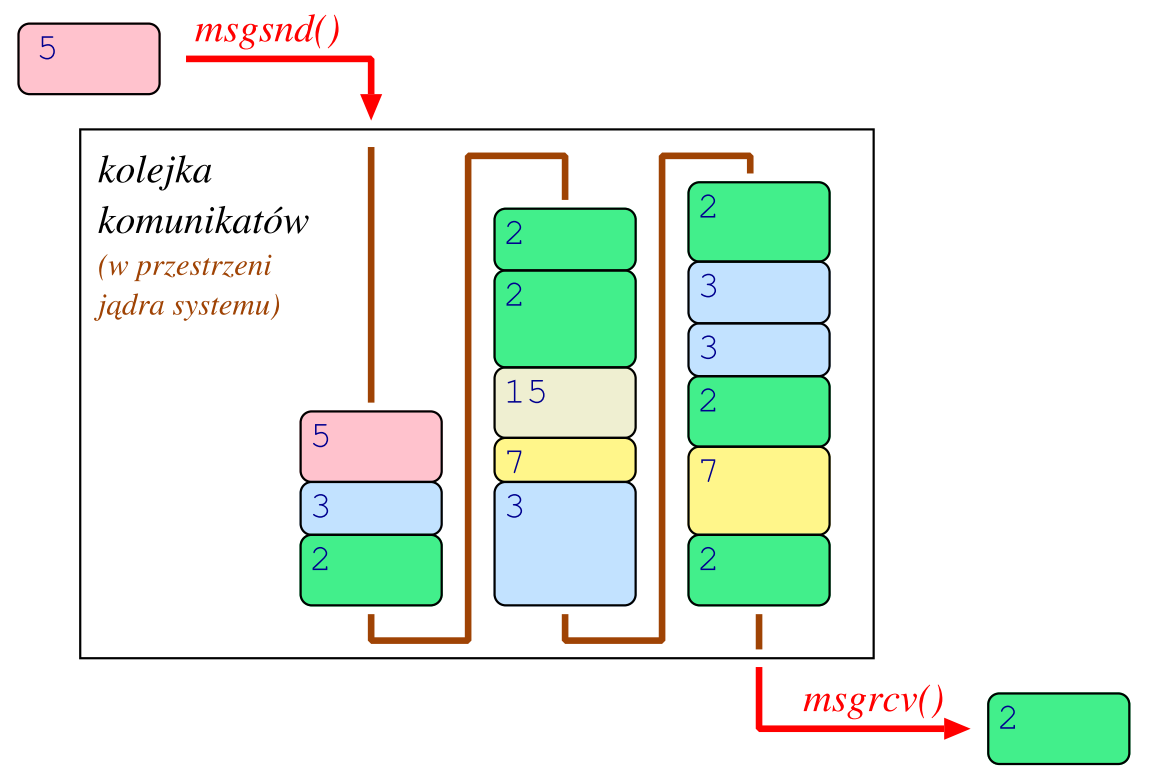
\includegraphics[width=0.8\textwidth]{s6_int_kolejka.png}
\caption{Kolejka komunikatów}
\end{figure}

\subsection{Funkcja select}

\subsection{Semafory}

chroniona zmienna systemowa, operacje atomowe V (inc), P (dec), nie może być < 0, synchronizacja procesów

\subsection{Pamięć współdzielona}

jeden proces tworzy obszar pamięci RAM, pozostałe mają do niego dostęp -- wspólny segment pamięci, odwzorowana jako własny obszar pamięci logicznej, wymaga dodatkowej synchronizacji

\subsection{Zmapowany plik w pamięci}

\subsection{Przekazywanie komunikatów}

RPC -- zdalne wywoływanie procedur
RMI -- technologia Java, stub
COBRA -- komunikacja między różnymi językami
MPI -- obliczenia wielowątkowe
\clearpage
\section{S7 -- Protokoły Internetu, Ochrona danych i uwierzytelnianie w Internecie}

\clearpage
\section{S8 -- Spójność sieciowego systemu operacyjnego}

%nie ma spójności, tylko halucynacje i śmierć z niedożywienia

System sieciowy składa się z wielu stacji roboczych i serwerów połączonych siecią. System sieciowy zawiera komponenty pozwalające na współdziałanie pomiędzy stacjami roboczymi a serwerami. Użytkownik jest świadomy że pracuje w sieci złożonej z wielu komputerów. Stosowana jest wspólna struktura komunikacji. Sieciowy system operacyjny tworzy środowisko w którym użytkownicy mają dostęp do wspólnych zasobów.
 
\textbf{Właściwości:}

\begin{itemize}
	\item Luźno powiązany sprzęt - różnego typu stacje robocze i serwery połączone siecią LAN.
	\item Różne systemy operacyjne - UNIX, Windows
	\item Obliczenia wykonywane przeważnie na maszynie lokalnej
	\item Pewien zbiór wspólnych usług i protokołów współpracy – wspólne serwery plików, poczta elektroniczna, TCP/IP
\end{itemize}
 
Popularne sieciowe systemy dostępne na rynku to:
\begin{itemize}
    \item Windows Server 2012 R2
    \item NetWare
    \item Unix
    \item Linux
\end{itemize}

Komunikacja sieciowa w sieciowym systemie operacyjnym jest oparciu o sieć magistrali, pierścienia lub gwiazdy. Obsługa komunikacji zgodnie z modelem ISO/OSI (siedem warstw) przy użyciu TCP/IP. Większość komunikacji odbywa się w modelu klient-serwer. 

\textbf{Stosowane mechanizmy:}

\begin{itemize}
    \item NFS -- protokół oparty na UDP lub TCP. Jest standardowym sieciowym systemem plików w systemach uniksowych. Z NFS wiąże się wiele problemów -– przede wszystkim bardzo trudno zapewnić, że dana operacja została wykonana.
    \item SMB --  protokół służący udostępnianiu zasobów komputerowych, m.in. drukarek czy plików. SMB jest protokołem typu klient-serwer, a więc opiera się na systemie zapytań generowanych przez klienta i odpowiedzi od serwera. 
    \item Microsoft DFS -- implementacja rozproszonego systemu plików firmy Microsoft. Do wymiany danych korzysta on z protokołu SMB. DFS był już obecny w Windows NT 4.0, obecnie jest dostępny też w Windows Server 2000/2003/2008 oraz Samba 3.0.
	\item DFS – Pozwalają na rozproszenie danych po wielu lokalizacjach fizycznych (serwerach) przy zintegrowaniu lokalizacji logicznej. Mimo że pliki są rozrzucone po wielu serwerach plików, dla użytkownika otoczenia sieciowego mogą być one widoczne na jednym serwerze plików tyle, że np. w wielu katalogach. Dzięki temu:
	\begin{itemize}
		\item   zmniejsza się ryzyko utraty i zwiększa dostępność danych przy awarii jednego serwera,
		\item   dzieli się obciążenie na wiele różnych maszyn,
		\item  przy użytkownikach rozproszonych w wielu lokalizacjach można skierować ruch od nich do najbliższych im serwerów (odległość interpretując jako np. czas dostępu czy przepustowość sieci).
		\item Zalety DFS
		\begin{itemize}
			\item Zwielokrotnienie -- (z ang. replication) wiele kopii danych.
			\item Niezawodność -- wielokrotność egzemplarzy może uchronić przed ich zaginięciem.
			\item Efektywność -- szybszy i łatwiejszy dostęp do danych.
		\end{itemize}
		\item Wady DFS:
		\begin{itemize}
			\item Problemy ze spójnością.
			\item Edycja danych na jednym serwerze nie gwarantuje ich zmiany na pozostałych.
			\item Konieczny jest mechanizm zapewniający aktualizację na pozostałych serwerach.
			\item Optymalne rozmieszczenie serwerów sprzyja spójności danych.
		\end{itemize}
	\end{itemize}
	\item Zdalne wywoływanie procedur RPC (ang. Remote Procedures Calls) – mechanizm pozwalający programiście na wysyłanie pytań do serwera i otrzymywani od niego odpowiedzi. Protokoły realizujące tę procedurę, same realizują całość komunikacji, na którą składa się serwer (nasłuchuje na danym porcie i czeka na pytanie od klienta, odpowiada klientowi żądanymi danymi bądź kodem błędu), klient (nawiązuje połączenie z klientem i wysyła zapytanie do serwera pytanie w wcześniej zdefiniowanym formacie). Z punktu widzenia programisty, proces ten wygląda tak jakby wywoływał procedurę lokalnie.
	\item Komunikacja sieciowa w oparciu o sieć magistrali, pierścienia lub gwiazdy. Obsługa komunikacji zgodnie z modelem ISO/OSI (siedem warstw) przy użyciu TCP/IP. Większość komunikacji odbywa się w modelu klient-serwer.

\end{itemize}

\textbf{Sposoby dostępu do danych, organizacja pamięci podręcznej w SSO:}

Po otwarciu pliku znajdującego się na serwerze, na komputerze klienta, kopia tego pliku trafia do pamięci podręcznej na maszynie lokalnej. Dzieje się tak ze względu na oszczędność komunikacji sieciowej, która w tym przypadku mogłaby być „wąskim gardłem” w korzystaniu z SSO. Takie rozwiązanie problemu generuje inne problemy, tzn.: jak aktualizować plik na serwerze i czy plik aktualnie przez nas używany jest aktualny (gdyż do danego pliku może mieć dostęp więcej niż jeden użytkownik).
 
\textbf{Aktualizacja danych na serwerze:}

Podczas pracy z plikiem często należy zapisywać ten plik aby w razie awarii maszyny, nie utracić swojej pracy, dlatego wyróżnia się kilka sposobów aktualizacji pliku po stronie serwera:
\begin{itemize}
	\item pisanie natychmiastowe – rozwiązanie polegające na ciągłym zapisywaniu każdej kolejnej zmiany od razu na serwerze. Rozwiązanie te jest bardzo nieefektywne, gdyż powoduje, że komunikacją przez sieć jest praktycznie ciągła, ale jest najbezpieczniejszą metodą
	\item pisanie opóźnione – zmiany zapisywane są najpierw w pamięci podręcznej, zaś później na serwerze (zazwyczaj po kliknięciu „Zapisz”). Rozwiązanie o wiele lepsze pod względem wydajności, aczkolwiek mniej niezawodne niż pisanie natychmiastowe
	\item okresowy przegląd – zapisywanie zmian na serwerze po upłynięciu jakiegoś ustalonego czasu (np. 1 minuty)
	\item pisanie przy zamknięciu – zapisywanie zmian na serwerze dopiero po zamknięciu pliku
\end{itemize}

\textbf{Spójność plików:}

Pracując w systemie gdzie do jednego pliku dostęp może mieć więcej niż jeden użytkownik, może generować problem z tym czy nasza aktualna kopia pliku na którym pracujemy jest aktualna. Jest kilka sposobów zapewniających omawianą spójność plików w sieciowym systemie operacyjnym:

\begin{itemize}
	\item odpowiedzialność po stronie serwera klienta – technika polegająca na czasowym odpytywaniu serwera czy nasza wersja pliku jest aktualna. Im większa częstotliwość tych zapytań, tym większa niezawodność, ale mniejsza wydajność
	\begin{itemize}
		\item Przy każdym dostępie do danych lub co stały okres czasu.
		\item Klient wysyła dużo komunikatów do serwera -- skutkuje zwiększeniem się ruchu sieciowego.
		\item Możliwe obciążenia serwera.
	\end{itemize}
	\item odpowiedzialność po stronie serwera – w tym wypadku to serwer pamięta z których plików i którzy użytkownicy aktualnie z nich korzystają. Po każdej aktualizacji pliku, serwer powiadamia o tym klientów o tym, że ich kopie są nieaktualne
	\begin{itemize}
		\item Serwer monitoruje stan wszystkich plików.
		\item Klient informuje o zmianach w plikach.
		\item Wszystkie kopie można odczytywać w tym samym czasie.
		\item Tylko jedna kopia może być modyfikowalna.
	\end{itemize}
\end{itemize}

\clearpage
\section{S9 -- Charakterystyka mikrokontrolerów}

Mikrokontroler to układ scalony mikroprocesorowy, który zawiera elementy, takie jak: jednostkę centralną (CPU), pamięć (danych, programu) oraz układy wejścia/wyjścia. Jego nazwa pochodzi od obszaru zastosowań -- sterowanie urządzeniami elektronicznymi. Bloki funkcjonalne, jakie może zawierać to: 
\begin{itemize}
\item kontrolery przerwań,
\item generator sygnału zegarowego (np. oscylator),
\item układy licznikowe,
\item kontrolery transmisji,
\begin{itemize}
\item równoległej,
\item szeregowej,
\end{itemize}
\item przetworniki analogowo-cyfrowe oraz cyfrowo-analogowe,
\item zegar czasu rzeczywistego (RTC),
\item watchdog (układ wykrywający błędne działanie systemu, zapobiega awariom -- zabezpiecza przed zawieszeniami),
\item etc.
\end{itemize}
Elementy te odróżniają mikrokontroler od mikroprocesora. Układ ten jest zdolny do autonomicznej pracy.

Mikrokontrolery wykorzystują następujące rodzaje pamięci:
\begin{itemize}
\item EPROM -- nieulotna, można je podzielić na jednorazowo programowalne (OTP) lub wielokrotnie, z możliwością kasowania dotychczasowej zawartości (EPROM), używana jest do pamięci programu (ale rzadko)
\item EEPROM -- nieulotna, kasowana elektrycznie, podobnie jak powyższa, stosowana jest do pamięci programu
\item flash -- nieulotna, można ją programować bezpośrednio w mikrokontrolerze, również zawiera pamięć programu
\item SRAM -- statyczna pamięć RAM, czyli ulotna, używana jest do pamięci danych
\item FRAM -- nieulotne pamięci ferroelektryczne, zastosowane np. w moich ,,ulubionych'' MSP430
\end{itemize}

Architektury mikrokontrolerów można podzielić ze względu na dostęp do pamięci lub typu listy instrukcji. Zgodnie z wiedzą z Architektury Komputerów wiemy, że istnieją architektury podzielone ze względu na dostęp do pamięci jak: von Neumanna, harvardzka, mieszana.

Architektura von Neumanna cechuje się tym, że ta sama pamięć przechowuje program oraz dane. Dostęp do nich odbywa się przez jedną, wspólną magistralę, a każda komórka posiada unikatowy adres. Kolejnym elementem jest jednostka sterująca, która jest odpowiedzialna za pobieranie i przetwarzanie instrukcji oraz danych trzymanych w tej pamięci.

Architektura harvardzka wyróżnia dwa rodzaje pamięci -- na program oraz na dane. W odróżnieniu od poprzedniej architektury, ta pozwala na równoległą komunikację z pamięciami programu oraz danych, ponieważ występują tu osobne magistrale.

Architektura mieszana wyróżnia dwa rodzaje pamięci, jak w architekturze harvardzkiej, jednak z jedną magistralą, jak w architekturze von Neumanna.

Drugim podejściem do podziału na architektury jest podział na listy instrukcji. Pierwszą z nich jest CISC (\textit{Complex Instruction Set Computing}). Zbiór rozkazów jest złożony, wykonanie instrukcji wymagają od kilku do kilkunastu cykli zegara. Duża liczba trybów adresowania oraz liczba rozkazów powodują, że układy dekoderów są skomplikowane. W tej architekturze rozkazy operują bezpośrednio na pamięci.

Innym podejściem jest architektura RISC (\textit{Reduced Instruction Set Computing}). Posiada ona więcej rejestrów w stosunku do CISC, aby zmniejszyć narzut komunikacji z pamięcią. Tryby adresowania zostały zredukowane, aby zmniejszyć stopień skomplikowania dekoderów. 

Mikrokontrolery są zdolne do autonomicznej pracy, dzięki dostępnym peryferiom, które wspomagają kontrolę urządzeń zewnętrznych. Można do nich zaliczyć:
\begin{itemize}
\item układ licznika w najprostszej postaci jest rejestrem przesuwnym, ważną cechą tego układu jest jego pojemność (np. 8 bit)
\item oscylatory generujące sygnały zegarowe, oprócz nich można podłączyć do $\mu$C zewnętrzne układy
\item watchdog -- ważnym elementem pracy $\mu$C, ponieważ przywraca działanie układu do normalnego trybu w razie, gdy mikrokontroler przestanie działać poprawnie
\item przetworniki analogowo-cyfrowe pozwalające na pracę z analogowymi peryferiami (np. czujnikami temperatury); przetworniki cyfrowo-analogowe pozwalają generować analogowe sygnały na podstawie cyfrowych danych
\end{itemize}

System przerwań opiera się na sygnałach, które powodują zmianę przepływu sterowania, niezależnie od wykonywanego programu. Przerwanie potrafi wstrzymać aktualnie wykonywany program i wykonać odpowiedni kod do obsługi danego przerwania. Pozwala to na interakcję z podłączonymi urządzeniami (np. przetwarzanie danych, gdy się pojawią), lub obsługę licznika.

Mikrokontrolery pozwalają na komunikację z zewnętrznymi urządzeniami. Niektóre z nich mogą mieć konkretny interfejs komunikacyjny. W $\mu$C najważniejszym interfejsem są piny GPIO, które umożliwiają komunikację, ich zachowanie programowane jest przez programistę, domyślnie nie mają określonego zastosowania. Mogą być zastosowane do implementacji interfejsów -- np. USART, SPI, I$^{2}$C. 

USART pozwala na szeregową komunikację z zewnętrznymi urządzeniami. Komunikacja ta może być synchroniczna lub asynchroniczna. Ta forma transmisji jest wykorzystywana w standardach RS232, RS485 (różnią się poziomami logiki). W trybie synchronicznym wykorzystywana jest dodatkowa linia zegara synchronizującego. Magistrala ta wymaga dwóch linii transmisyjnych (RX -- odbiór, TX -- wysyłanie).

I$^{2}$C jest inną magistralą szeregową, pozwala na podłączenie wielu urządzeń. Urządzenia podzielone są na dwie klasy -- master oraz slave. Master generuje sygnał zegarowy, rozpoczyna komunikację z podwładnymi urządzeniami. Węzły slave odbierają sygnały zegarowe oraz odpowiadają, gdy komunikacja jest zaadresowana do nich. Magistrala ta wymaga dwóch linii sygnałowych (dane, sygnał zegara).

Inną magistralą komunikacyjną jest SPI. Ona również zezwala na podłączenie wielu urządzeń. Zezwala na komunikację full-duplex, czyli urządzenia mogą się ze sobą komunikować równocześnie. Podobnie jak I$^{2}$C, posiada podział na master oraz slave. Wymaga trzech linii komunikacyjnych (sygnał zegara, wyjście danych układu master, wejście danych układu master) oraz jedną linię komunikacyjną na urządzenie (master posiada linie wyboru układu slave).

Programowanie mikrokontrolerów może odbywać się:
\begin{itemize}
\item szeregowo w systemie (ISP), poprzez SPI
\item przez bootloader -- w układach, które mają możliwość modyfikacji programu, przesyłanie może odbyć się np. przez UART
\item przez JTAG -- wykorzystywane do programowania i debugowania, początkowo służył do weryfikacji poprawności montażu układów scalonych
\end{itemize}
Układy można skonfigurować przy pomocy lock bitów (zabezpieczają przed nieuprawnionym dostępem do pamięci programu) oraz fuse bitów (konfiguracja układu, źródeł sygnału zegarowego, watchdoga, etc.).

Mikrokontrolerów zazwyczaj nie posiadają systemu operacyjnego, chociaż istnieją rozwiązania RTOS (np. uClinux, freeRTOS). Programowanie zwykle wykorzystuje asemblera bądź C ze wstawkami asemblera. Konwencja tworzenia programów na mikrokontrolery opiera się na tym, że procesor powinien wykonywać zadania, mimo wystąpienia zdarzeń losowych, czy też podczas oczekiwania na jakieś przerwanie. W niektórych zastosowaniach może być ważne również usypianie i wybudzanie mikrokontrolera w celu oszczędzania zasilania, gdy $\mu$C oczekuje na np. dane.
\clearpage
\section{S10 -- Systemy wbudowane w strukturach programowalnych}

Przypomnienie -- \textbf{struktury programowalne} to układy elektroniczne, które mają programowalną strukturę, mogą działać jak dowolny układ cyfrowy (o ile zasoby na to zezwalają). Funkcjonalność jest definiowana przez programistę, a nie producenta, co pozwala zmniejszyć koszty, bo z punktu widzenia producenta, produkowane układy są identyczne. PLD są programowane za pomocą języków opisu sprzętu (najpopularniejsze -- Verilog, VHDL), a narzędzie syntezy przetwarza kod programu na fizyczne połączenia. Wyróżnia się układy PLD takie jak: 
\begin{itemize}
\item SPLD -- PLA, PLE, PAL; najprostsze, mają ograniczone możliwości funkcjonalne i logiczne,
\item CPLD -- koncepcyjnie podobne do SPLD, ich architektura opiera się na makrokomórkach, które tworzą bloki funkcyjne, łączone są przez matrycę połączeń,
\item FPGA -- najbardziej zaawansowane, składają się z CLB łączonych w bloki, łączone są przez linie traktów połączeniowych.
\end{itemize}
Więcej informacji można znaleźć w punkcie K9, nie ma się co tu rozpisywać więcej, bo ileż tu można upchnąć ciekawych informacji \texttt{:-)))}.

\textbf{System wbudowany} -- system komputerowy o specjalnym przeznaczeniu, jest integralną częścią obsługiwanego przez niego sprzętu. System ten spełnia wymagania, które zostały określone do zadań, które ma wykonywać. Tak więc zgodnie z tą definicją komputer osobisty nie jest systemem wbudowanym. Systemy wbudowane wykorzystują mikroprocesory bądź mikrokontrolery, które są zaprogramowane do wykonywania tylko i wyłącznie tychże zadań (mają dedykowane oprogramowanie) -- dlatego są nazwane systemami szczególnego przeznaczenia. Systemy te można także oprzeć na strukturach programowalnych. Dzięki wyspecjalizowaniu tych systemów, pobierają one mniej energii, mają mniejsze rozmiary w stosunku do systemów ogólnego przeznaczenia. Systemy te także cechują się wysoką niezawodnością -- są odporne na awarie i zakłócenia.

Z systemami wbudowanymi można się spotkać na każdym kroku. Występują one m.in. w:
\begin{itemize}
\item komputerach pokładowych (w aucie, samolocie, etc.), 
\item systemach naprowadzania rakiet (\texttt{;-)}),
\item sprzęcie medyczny,
\item bankomatach,
\item ,,yntelygentnych'' urządzeniach (telewizory, lodówki, boję się pomyśleć co jeszcze),
\item routerach,
\item systemach alarmowych,
\item drukarkach,
\item odtwarzaczach DVD/Blu-Ray/etc.,
\item można tak wymieniać do wieczora, ale chyba komisji to się zbytnio nie spodoba.
\end{itemize} 

System wbudowany składa się z trzech głównych części:
\begin{itemize}
\item obwody wejściowe (czujniki, przetworniki A/C lub C/A, etc.) -- zbierają dane,
\item jednostka centralna -- pobiera dane, przetwarza je przez swój algorytm oraz przekazuje na obwody wyjściowe,
\item obwody wyjściowe -- mogą to być porty komunikacyjne, czy też wyjścia sterujące.
\end{itemize}

Realizacja systemów wbudowanych na strukturach programowalnych może się odbyć na CPLD lub FPGA (SPLD nie są wystarczająco duże).

Układy CPLD oraz FPGA można zaprogramować programowymi procesorami. Jednym z nich, dosyć popularnym jest PicoBlaze, (8-bitowy). Jest on stworzony w HDLu. Posiada on cechy podobne do istniejących na rynku mikrokontrolerach (takich jak: 8051, ATtiny13, ST6215). W odróżnieniu od nich, pozwala na dowolną liczbę peryferii, ograniczeniem jest liczba bloków wybranego PLD.

Istnieją także inne mikroprocesory, którymi można zaprogramować układy PLD, jednakże wymagają one FPGA (nie CPLD). Są to: MicroBlaze, OpenRISC, ARM Cortex-M1 (oczywiście, jest ich więcej). MicroBlaze jest podobny do PicoBlaze, jednak jest to procesor programowy 32-bitowy, posiada większą liczbę zasobów, oraz wyposażony w jednostkę FPU (czyli obsługuje nasze ulubione liczby zmiennoprzecinkowe). Z ciekawostek, obsługa MicroBlaze jest zawarta w kodzie źródłowym jądra Linuksa.

Programowanie takich procesorów programowych odbywa się w dwóch etapach. Pierwszy z nich polega na definicji układu przy pomocy HDLa -- tutaj jest ustalana ,,budowa'' procesora. Następnie jest to przekształcane na sprzętową implementację jako układy kombinacyjne lub sekwencyjne. Kolejny krok to stworzenie kodu programu w Asemblerze bądź C/C++, a następnie zaprogramowanie procesora.

Łączenie mikroprocesorów i układów programowalnych może się odbyć na cztery sposoby:
\begin{enumerate}
\item \textbf{Mikroprocesor/mikrokontroler}

Połączenie mikroprocesora z peryferiami w jeden lub kilka układów scalonych.
\item \textbf{$\mu$procesor/$\mu$kontroler + PLD}

Rozwiązanie to pozwala rozszerzać systemy procesorowe o dodatkowe możliwości, które dają układy programowalne.
\item \textbf{PLD zintegrowane z $\mu$procesorem / inaczej: $\mu$kontroler z wbudowaną częścią FPGA w jednym układzie scalonym}

Układy PLD z wbudowanym procesorem, np. Xilinx Virtex II + PowerPC. Rozwiązanie to nie przyjęło się ze względu na wysoką cenę.

\item \textbf{Układy PLD z zaimplementowanym $\mu$procesorem}

Rozwiązanie używane do projektowania i weryfikacji projektów przez firmy produkujące układy scalone. Wraz ze wzrostem wydajności i pojemności tańszych układów ta konfiguracja zaczyna być konkurencyjna dla mikrokontrolerów. Rozwiązanie to wydaje się być optymalne dla sprzętowych procesorów (PicoBlaze, MicroBlaze, etc.).
\end{enumerate}

Układy programowalne dają elastyczność, struktura systemu wbudowanego o taki układ może być dostosowana ściśle do potrzeb oraz może być w prosty sposób zmieniona. Gotowe mikroprocesory nie pozwalają na manipulację liczbą portów czy możliwych peryferii do podłączenia. Można zbudować system oparty o wiele procesorów, gdzie każdy ma przydzielone inne zadanie do wykonania. 

Wadą takiego rozwiązania jest większy pobór mocy.

Układy programowalne pozwalają na zrealizowanie dowolnych peryferii wewnątrz układu, np. układy DVB, szyfrujące, bloki przetwarzania sygnałów, porty szeregowe i równoległe, magistrale, etc.

\clearpage

\part{Pytania specjalnościowe -- INS}
\section{S1 -- Konfiguracja sieciowa systemów operacyjnych (sterowniki urządzeń sieciowych, ustawienia parametrów sieci lokalnej i TPC, automatyzacja konfiguracji)}

Sieciowy system operacyjny to system, którego jądro ma zintegrowany stos sieciowy.
Mądrze brzmi, ale co to znaczy?
Znaczy to tyle, że jądro takiego systemu posiada
\begin{itemize}
	\item{sterowniki obsługujące karty sieciowe,}
	\item{oprogramowanie obsługi co najmniej trzech najniższych warstw, tj. łącza danych, sieciowej i transportowej}
	\item{funkcje biblioteczne wspierające gniazdka Berkeley, Windows bądź interfejs TLI.}
\end{itemize}

\subsection{Urządzenia}
W systemie możemy wyróżnić między innymi następujące trzy rodzaje urządzeń.

\begin{itemize}
	\item{Znakowe -- są to urządzenia, które obsługują odczyt i zapis znak po znaku. Nie są buforowane i interakcja jest natychmiastowa. Przykład: drukarka.}
	\item{Blokowe -- urządzenia te umożliwiają odczyt i zapis całych bloków. Są buforowane i umożliwiają dostęp do danych w nich przechowywanych. Przykład: dysk, plik.}
	\item{Interfejsy sieciowe -- zamiast znaków czy bloków, obsługują pakiety.}
\end{itemize}

Każde z tych urządzeń jest obsługiwane przez odpowiedni sterownik -- część jądra systemu, odpowiedzialną za obsługę urządzeń.
Sterowniki można dołączać do jądra \textbf{statycznie -- } w trakcje kompilacji -- oraz \textbf{dynamicznie -- } w formie ładowalnych modułów.

Interfejsy można konfigurować lokalnie, za pomocą plików konfiguracyjnych i narzędzi typu ifconfig.
Jednak istnieją również rozwiązania pozwalające na automatyczną konfigurację systemu w momencie jego uruchomienia i włączenia do sieci.

\subsection{BOOTP}
Jest to protokół służący do konfiguracji komputerów.
Taki komputer po uruchomieniu rozsyła na adres rozgłoszeniowy zapytanie BOOTP.
Kiedy serwer odbierze to zapytanie, wysyła klientowi odpowiedź BOOTREPLY zawierającą konfigurację.

Tego protokołu używano również do pobierania obrazu systemu operacyjnego.
Pozwalało to na używanie prostych terminali, które nie posiadały własnych dysków, a całość konfiguracji ściągały z sieci i ładowały do pamięci operacyjnej.

\subsection{DHCP}
Następcą BOOTP, jest protokół DHCP (Dynamic Host Configuration Protocol).
W odróżnieniu do BOOTP, protokół ten jest przeznaczony dla maszyn posiadające własne dyski i skupia się na automatycznej konfiguracji komputerów, które często mogą zmieniać swoją fizyczną lokalizację.
Potrafi komunikować się z komputerem również po uruchomieniu się systemu, a nie tylko przed, dzięki czemu łatwiejsze staje się odnawianie dzierżawy adresu -- komputera nie trzeba uruchamiać ponownie.
\clearpage
\section{S2 -- Mechanizmy zdalnego dostępu do zasobów sieciowych (dyski sieciowe, mapowanie uprawnień dostępu, sieciowe zarządzania użytkownikami NIS/LDAP)}

Udostępnianie zasobów w sieci jest bardzo wygodnym rozwiązaniem.
Zwalnia nas z potrzeby wymieniania się nośnikami danych i kopiowania danych między komputerami.
Rozwiązań jest wiele i od naszych wymagań czy możliwości zależy to, które wybierzemy.

\subsection{FTP}
Jedną z najbardziej rozpowszechnionych usług tego typu są serwery FTP oraz ich bezpieczne odpowiedniki SFTP (tunelowanie ssh) oraz FTPS (ssl/tls).

FTP (File Transfer Protocol) jest to usługa, która pozwala nam na udostępnienie miejsca na serwerze, z którego ludzie mogą pobierać lub wysyłać dane.
Może ona działać w dwóch trybach, z których oba potrzebują dwóch połączeń -- do przesyłania poleceń oraz danych.
Tryby te to
\begin{itemize}
	\item{aktywny -- gdy klient łączy się do serwera i wymienia polecenia, a dopiero później ustanawia nowe połączenie na porcie N+1 w celu przesłania danych,}
	\item{pasywny -- gdy klient od samego początku ustanawia oba połączenia.}
\end{itemize}

\subsection{NAS}
Będąc w temacie zasobów sieciowych nie można oczywiście pominąć dysków sieciowych.
Są to urządzenia wpinane do sieci -- zazwyczaj kablem ethernetowym -- lecz dla użytkowników są widoczne jak zasoby lokalne.
Daje nam to możliwość udostępnienia zasobów raz -- nie musimy wymieniać się nośnikami i kopiować danych.

\subsection{NFS}
Jednak nie trzeba w celach udostępniania danych w sieci kupować dedykowanych urządzeń. 
Można skorzystać z protokołu NFS, który umożliwia udostępnienie swoich danych w sieci.
Udostępnione pliki można zamontować w swoim systemie i operować jak na zasobach lokalnych.

\subsection{SMB}
Innym protokołem jest SMB.

\subsection{Uprawnienia}
NFS musi oczywiście sprawdzić, czy mamy uprawnienia dostępu do zasobów, co sprowadza nas do tematu uprawnień i zarządzania użytkownikami.
W przypadku NFSa, system sprawdza czy nasz użytkownik i jego uprawnienia zgadzają się z tym co jest na serwerze -- jeśli spróbujemy odczytać coś do czego nasz użytkownik nie ma dostępu to się nam to nie uda.
Konfigurację przeprowadza się za pomocą pliku /etc/exports.

\subsection{Zarządzanie użytkownikami}
Dla zarządzania użytkownikami również istnieją różne rozwiązania, m.in. \textit{NIS, LDAP} czy \textit{Active Directory.}

NIS (Yellow Pages) jest protokołem umożliwiającym współdzielenie informacji o użytkownikach.
Działa on w architekturze serwer-klient, gdzie serwer posiada bazę z informacjami na temat użytkowników, a klient z tej bazy może skorzystać.
Można więc tak ustawić sieć, że gdy użytkownik próbuje się zalogować do komputera, a w lokalnym systemie nie widzimy takiego użytkownika, komputer odpytuje serwer z bazą danych i na tej podstawie weryfikuje czy użytkownik może uzyskać dostęp.

NIS ma jednak tę wadę, że klient może pobrać całą bazę, a następnie przeprowadzić atak siłowy celem złamania haseł.

Następnikiem NISa jest LDAP.
LDAP podobnie jak NIS działa w architekturze serwer-klient, jednak różnica polega na tym, że weryfikacja odbywa się po stronie serwera.

Przykładem, gdzie takie rozwiązanie jest wdrożone może być sama politechnika.
Studenci posiadają konta na poczcie, którego można użyć do zalogowania się do sieci Eduroam.
Takie rozwiązanie jest również wdrożone w niektórych laboratoriach.
\clearpage
\section{S3 -- Metody rozwiązywania problemu martwego punktu (impasu) w systemach i sieciach komputerowych}

Impas, inaczej zakleszczenie, jest pojęciem znanym z programowania współbieżnego.
Jest to sytuacja, w której procesy, bądź wątki czekają na siebie nawzajem i żadna z tych operacji nie może zostać ukończona.

Do takiej sytuacji może dojść np. w przypadku, gdy proces A żąda zasobu, który jest zajęty przez proces B, a proces B żąda zasobu zajętego przez proces A.
Wychodzi wtedy cykliczna zależność, która blokuje system.

Pojęciem powiązanym z zakleszczeniem jest \textit{zagłodzenie.}
Przykładem jest \textit{problem ucztujących filozofów.}
Problem polega na tym, że procesy wymagają do działania dwóch zasobów -- widelców.
Jeśli jeden filozof zacznie jeść, to dwaj obok niego automatycznie nie mogą jeść.

Metody walki z tym problemem dzielą się na
\begin{itemize}
	\item{wykrywanie i likwidację,}
	\item{zapobieganie,}
	\item{unikanie.}
\end{itemize}

\subsection{Wykrywanie i likwidacja}
Polega na cyklicznym sprawdzaniu stanu systemu i wykrywaniu czy nie pojawiły się w nim blokady.
W przypadku ich wykrycia, system może odłączać poszczególne zasoby od puli zasobów zajętych, aż do momentu usunięcia blokady.
Takie podejście jest oczywiście zarezerwowane dla systemów, w których istnieje możliwość wywłaszczenia zasobów.

\subsection{Zapobieganie (statyczne)}
Do wystąpienia blokady, konieczne jest spełnienie czterech warunków
\begin{itemize}
	\item{wyłączność -- zasoby nie mogą być współdzielone (w danej chwili zasób może być wykorzystywany tylko przez jeden proces,}
	\item{niewywłaszczalność -- zasób nie może zostać odebrany procesowi przed zakończeniem operacji,}
	\item{przetrzymywanie i czekanie -- procesy zajmują zasób i oczekują na kolejny,}
	\item{cykliczne oczekiwanie -- istnieje cykl procesów oczekujących na siebie wzajemnie.}
\end{itemize}

Aby zapobiegać blokadom, należy tak projektować system, by przynajmniej jeden z tych warunków nie został spełniony, tj.

\begin{itemize}
	\item{pozwolić na jednoczesny dostęp do zasobów lub sprawić, by procesy nie korzystały z tych samych zasobów,}
	\item{pozwolić na wywłaszczenie zasobów,}
	\item{wymuszenie, by proces zajął wszystkie potrzebne mu zasoby albo nic,}
	\item{}
\end{itemize}

\subsection{Unikanie (dynamiczne)}
Podczas gdy zapobieganie blokadom opiera się na rozwiązaniach statycznych, tj. implementowanych przy projekcie systemu, unikanie blokad wykorzystuje aktualne dane o stanie systemu, co pozwala odpowiednio zareagować.

\subsubsection{Algorytm bankiera}
Pozwalamy procesowi na zajęcie zasobu, jeśli po jego zajęciu będzie istniała możliwość uporządkowania procesów tak, by uniknąć blokady.

Porządkowanie zasobów dla procesów w ogólnym przypadku jest problemem \textbf{NP-zupełnym,} co znaczy, że nie jest to łatwe zadanie, a heurystyczne algorytmy mogą odrzucać część prawidłowych stanów.

\subsection{Scentralizowane i rozproszone}
Algorytmy można dzielić ze względu na różne kryteria.
Jednym z takich podziałów jest podział na algorytmy scentralizowane oraz rozproszone.

\subsubsection{Scentralizowane}
Są to algorytmy opierające się na znajomości stanu globalnego systemu.
\subsubsection{Rozproszone}
Są to algorytmy opierające 

\subsection{Optymalne i suboptymalne}
Algorytmy można również dzielić na
\begin{itemize}
	\item{optymalne -- algorytm doskonale sobie radzi i odrzuca jedynie stany niebezpieczne,}
	\item{suboptymalne -- jest możliwe, że algorytm odrzuci część stanów bezpiecznych.}
\end{itemize}


\clearpage
\section{S4 -- Metody równoważenia obciążeń w systemach i sieciach komputerowych}

Równoważenie obciążenia w systemach nie jest banalnym tematem.
Wiele procesów wymaga dostępu do zasobów, w tym do czasu procesora.

Za kolejkowanie procesów odpowiada \textbf{planista.}
Jest to proces, którego zadaniem jest między innymi przydzielenie procesom miejsca w kolejce.

\subsection{Rodzaje planistów}
Wyróżniamy planistów
\begin{itemize}
	\item{krótkoterminowych -- odpowiadających za procesy oznaczone jako \textit{gotowe,}}
	\item{średnioterminowych -- odpowiadających za ładowanie i usuwanie procesów z pamięci (swap),}
	\item{długoterminowych -- odpowiadających za uruchamianie nowych procesóœ.}
\end{itemize}

\subsection{Algorytmy planowania}
Same algorytmy, wg. których działać może planista możemy podzielić na wywłaszczeniowe oraz niewywłaszczeniowe.

\subsubsection{Algorytmy niewywłaszczeniowe}
To takie, które nie dopuszczają sytuacji, w której proces, który jest aktualnie obsługiwany, zostaje wywłaszczony -- przestaje się go obsługiwać przed zakończeniem.

Do takich algorytmów można zaliczyć kolejkowanie
\begin{itemize}
	\item{SJF - Shortest Job First,}
	\item{FIFO - First In First Out,}
	\item{LIFO - Last In First Out.}
\end{itemize}

\subsubsection{Algorytmy wywłaszczeniowe}
Te algorytmy pozwalają, a nawet opierają się na tym, że proces zostaje wywłaszczony.
Można tutaj wspomnieć między innymi o
\begin{itemize}
	\item{Round-robin -- każdy proces dostaje kwant czasu, po którego upływie zostaje wywłaszczony,}
	\item{Shortest Remaining Time -- proces zostaje wywłaszczony kiedy zjawi się proces, o krótszym czasie obsługiwania}
	\item{Podejście priorytetowe -- obsługiwany jest proces o najwyższym priorytecie.}
\end{itemize}


\clearpage
\section{S5 -- Źródła zagrożeń bezpieczeństwa systemów i usług informatycznych}

\subsection{Natura}
Jednym z zagrożeń dla systemów, które istnieje, a nie zawsze się o nim myśli jest natura.
Woda może zalać sprzęt, piorun uszkodzić instalacje, a zwierzątka poprzegryzać kable i należy się przed tym zabezpieczać.

\subsection{Użytkownicy}
Jednak głównym źródłem zagrożeń dla systemów są ludzie.
Nawet jeśli zaprojektujemy system, który w naszej opinii jest wyjątkowo dobrze zabezpieczony, to ktoś zawsze znajdzie sposób, by nam udowodnić, że się mylimy (czy to przez przypadek, czy umyślnie).

Użytkownicy ustawiają słabe hasła, które łatwo złamać, bądź też udostępniają je na lewo i prawo.
Robią coś i nie pomyślą nawet, że ich działania mogą przyczynić się do ujawnienia tajnych danych czy zakażenia komputera wirusem.

\subsection{Socjotechniki}
Ludzie są łatwowierni.
Jeśli wejdziemy do jakiegoś miejsca odpowiednio ubrani i będziemy sprawiać wrażenie, że dokładnie wiemy co robimy to nikt nas nie zatrzyma.
Można więc w okolice firmy podrzucić odpowiednio zakażony pendrive lub wysłać wiadomość podając się za przedstawiciela banku i poprosić o udostępnienie danych.

\subsection{Haksy}
Również ludzie w postaci programistów są odpowiedzialni za błędy w oprogramowaniu, które mogą pozwalać na nieautoryzowany dostęp do systemu.
Programiści mogą chcieć ułatwić sobie pracę tworząc tak zwane \textit{backdoory} i później ich nie usuwają (ponownie, specjalnie bądź przez przypadek).

Oczywiście poza przyczynami losowymi i czynionymi nieumyślnie mamy też do czynienia z niebezpieczeństwem ze strony ludzi, którzy umyślnie chcą spowodować szkody.
Do zagrożeń ze strony takich osób należą

\subsubsection{Sniffery}
Oprogramowanie podsłuchujące dane przepływające w sieci korzystając z faktu, że niestety internet był projektowany w czasach, gdy bezpieczeństwo w sieci nie było wielkim tematem i dane w niższych warstwach są przesyłane w postaci jawnej.
Wykrywanie ich polega na wykorzystaniu zasady działania snifferów -- wykorzystują one kartę sieciową przełączoną w tryb \textit{promiscuous,} aby przechwytywać pakiety, które nie są do nich adresowane.

Można więc taką kartę wykryć wysyłając do podejrzanego hosta pakiet ICMP ECHO z jego adresem IP, ale cudzym adresem MAC.
Praworządna karta nie powinna takiego pakietu przyjąć, lecz karta podsłuchująca wyśle odpowiedź i w ten sposób można poznać kto jest kto.

\subsubsection{Denial of Service}
Atak typu DoS polega na zajęciu zasobów systemowych (czas CPU, miejsce na dysku) w taki sposób, że inne procesy i użytkownicy nie są w stanie z nich korzystać.
Atak taki można również przeprowadzić z sieci, np. poprzez zasypywanie serwera pakietami.

Walczyć z takim atakiem można poprzez ustawienie limitów w systemie, np. limit na miejsce przeznaczone dla jednego użytkownika, czy liczbę procesów mogących operować jednocześnie.

\subsubsection{Spoofing}
Podszywanie się pod kogoś innego.
\begin{itemize}
	\item{DNS -- wysłanie do serwera DNS fałszywej informacji kojarzącej domenę z adresem IP.}
	\item{ARP -- rozsyłanie w sieci spreparowanych pakietów ARP zawierających fałszywe adresy MAC, co powoduje przesłanie danych w złe miejsce.}
\end{itemize}
\clearpage
\section{S6 -- Metody i mechanizmy zapewniania bezpiecznego dostępu i bezpiecznej komunikacji sieciowej w systemach komputerowych}

Temat bezpieczeństwa systemów i sieci należy zacząć od wspomnienia o najważniejszym elemencie bezpiecznego systemu, którym jest \textbf{użytkownik.}

Możemy zaprojektować najlepszy system, który będzie wykorzystywał najlepsze metody szyfrowania danych, lecz jeśli użytkownik nie będzie postępował zgodnie z zasadami, to system nigdy nie będzie bezpieczny.

Przykładowo możemy wymusić na użytkownikach, by używali długich i skomplikowanych haseł, jednak najprawdopodobniej doprowadzi to do zapisania takiego hasła gdzieś przy komputerze -- w takiej sytuacji tego hasła mogłoby równie dobrze nie być.

Opisane wyżej postępowanie nazywa się mianem \textit{bezpieczeństwa kosztem używalności.}
Takie postępowanie bardzo często prowadzi do zmniejszenia bezpieczeństwa systemu, a nie do jego ulepszenia.

Zanim przejdziemy dalej, powiedzmy sobie o trzech ważnych pojęciach.

\begin{itemize}
	\item{Identyfikacja -- przedstawienie systemowi swojej tożsamości, którą będzie on weryfikował w następnym kroku.}
	\item{Uwierzytelnianie -- polega na przedstawieniu systemowi pewnych dowodów, które przekonają go, że ,,rozmawia'' z odpowiednią osobą.}
	\item{Autoryzacja -- jest osobnym procesem i polega na otrzymaniu dostępu do zasobów lub usług systemu, a co za tym idzie, jest ściśle powiązana z uwierzytelnianiem.}
\end{itemize}

\subsection{Hasła}

Podstawowym mechanizmem zabezpieczania systemów są hasła.

\subsubsection{Hasła wielokrotnego użytku}
Najczęściej są one przechowywane w postaci zaszyfrowanej, a podczas uwierzytelniania hasło podane przez użytkownika przepuszczane jest np. przez funkcję skrótu i porównywane z wersją przechowywaną w systemie.
Jeśli system uzna, że hasła są zgodne to może udzielić dostępu.

Hasła tradycyjne mają tę wadę, że można je złamać, wykraść czy zgadnąć.
Dlatego, choć są wygodne, nie są najlepszą metodą zabezpieczania systemów.

\subsubsection{Hasła jednorazowe}
Alternatywą dla haseł tradycyjnych są hasła jednorazowe.

Przykładem mogą być hasła odczytywane z listy, która zawiera wcześniej wygenerowane hasła, wygasające po jednym użyciu.
Takie rozwiązanie obok haseł SMS często spotkać można w bankach.

Również w bankach można natknąć się na hasła generowane za pomocą tokenów.
Takie hasła zmieniają się automatycznie np. co 5 minut i ich ważność wygasa w momencie użycia.

\subsection{Szyfrowanie}
Równie ważnym tematem jest szyfrowanie danych.

Polega ono na zamianie danych z postaci jawnej do postaci zaszyfrowanej przy pomocy pewnego algorytmu szyfrującego i klucza, który będzie służył do odkodowania danych.

Metody szyfrowania możemy podzielić na symetryczne oraz asymetryczne.

\begin{itemize}
	\item{Symetryczne -- istnieje jeden klucz używany zarówno do szyfrowania i odszyfrowania.}
	\item{Asymetryczne -- istnieje para kluczy, z których jeden służy do szyfrowania, a drugi do odszyfrowania.}
\end{itemize}

Rozwiązanie asymetryczne stosuje się między innymi w GPG (Gnu Privacy Guard), które służy między innymi do szyfrowania i podpisywania korespondencji.
Kiedy dwie osoby chcą się komunikować za pomocą tej metody, generują dla siebie po parze kluczy, z których jeden jest określany mianem \textit{prywatnego} i jest znany tylko właścicielowi, a drugi jest kluczem \textit{publicznym,} który zostaje udostępniony.
Gdy ktoś zaczyna tworzyć maila, szyfruje go za pomocą klucza publicznego adresata.
Dzięki temu tylko osoba posiadająca klucz prywatny, pasujący do klucza publicznego, którym podpisana zostałą wiadomość, będzie w stanie ją  odczytać.

\subsection{Podpis}
Podpis cyfrowy ściśle wiąże się z opisanym wcześniej szyfrowaniem asymetrycznym.

Wykorzystuje się tutaj fakt, że wiadomość, którą da się odszyfrować kluczem publicznym, musiała zostać zaszyfrowana pasującym kluczem prywatnym. Co za tym idzie, została wysłana przez osobę posiadającą właśnie ten klucz prywatny.

Podpis cyfrowy służy do potwierdzania autentyczności pochodzenia wiadomości, ale także pozwala wykryć nieautoryzowane próby zmiany dokumentu.
\clearpage
\section{S7 - Różnice pomiędzy introspekcją i odzwierciedleniem – metodami stosowanymi do rozpoznania własności klas lub zmodyfikowania zachowania się aplikacji działających na wirtualnej maszynie Java}
\clearpage
\section{S8 -- Sposoby budowy i zarządzania aplikacjami rozproszonymi za pomocą pakietów należących do standardowej dystrybucji Javy}

Aplikacje rozproszone to takie, które są wykonywane na wielu maszynach celem rozłożenia obciążenia.

Takie aplikacje można zrealizować za pomocą zdalnego wywoływania metod obiektów, bądź przesyłania komunikatów.

\subsection{Gniazda}
Przesyłanie komunikatów wiąże się z wykorzystaniem gniazd sieciowych, a budowa aplikacji opiera się na architekturze klient-serwer.
Samą komunikację można podzielić na strumieniową (TCP) oraz datagramową (UDP).

Wygląda to tak, że zarówno klient jak i serwer otwierają gniazda sieciowe.
Następnie serwer oczekuje na nadejście nowych połączeń.
Klient podaje z jakim adresem IP chce się połączyć, a konkretna usługa jest rozpoznawana po numerze portu.
Gdy serwer odbierze połączenie, otwiera nowe gniazdo, przez które jest kontynuowana wymiana, a stare gniazdo istnieje w celach odbierania nowych połączeń.

\subsection{RMI}
Innym sposobem realizacji takiej aplikacji, który poznaliśmy w czasie studiów jest RMI.
RMI dostarcza mechanizmy pozwalające na udostępnianie oraz wywoływanie metod zdalnych obiektów.

Obiekty, których metody będą wywoływane zdalnie, przede wszystkim muszą implementować pewien konkretny interfejs.
Następnie, namiastka tych obiektów musi zostać zarejestrowana w rejestrze RMI.
Będzie ona służyła do wywoływania ich metod.

Kiedy klient chce wywołać metodę zdalnie, komunikuje się z rejestrem RMI i pobiera informacje o namiastkach i ich metodach.
Po pobraniu namiastek, może on działać na nich tak jakby to były zwyczajne obiekty lokalne -- komunikacja jest więc dla użytkownika niewidoczna.
\clearpage
\section{S9 -- Dostęp do internetowych baz danych na przykładzie wybranej technologii}
Internetowa baza danych to oczywiście baza danych dostępna w Internecie.
Bazy danych istnieją po to, by przechowywać dane w celu ich późniejszego wykorzystania.

\subsection{ORM}
Pojęciem niezwykle ważnym w tym temacie jest Mapowanie Obiektowo Relacyjne.
Pozwala ono na przetworzenie danych z postaci przechowywanej w bazie relacyjnej do postaci obiektów w wybranym języku programowania.

Pozwala to na dostęp do danych z zachowaniem wysokiego poziomu abstrakcji przy użyciu języka, z którym programiści są najlepiej obeznani.
Nie musimy więc pisać skomplikowanych zapytań SQLowych.
Wystarczy jedynie odwołać się do zmapowanych obiektów i ich metod, co jest wyjątkowo wygodne i pozwala na znaczne przyśpieszenie pisania aplikacji.

Ma to również tę zaletę, że odpowiedzialność za takie rzeczy jak odporność na SQL Injection przynajmniej częściowo zrzucamy na bibliotekę i jednocześnie w pewien sposób uniezależniamy się od konkretnej implementacji bazy danych -- to biblioteka dba o to, by odpowiednio przetłumaczyć nasze polecenia.

Jako że pytanie wyraźnie mówi o dostępie na przykładzie wybranej technologii, wypowiem się o tym jak to wygląda w Pythonie.

\subsection{DjangoORM}
Jednym z dostępnych rozwiązań w świecie Pythona jest DjangoORM.
Jest to system mapowania stworzony na potrzeby Frameworka webowego Django jednak po odpowiedniej konfiguracji można go używać bez części webowej.

Działa on w taki sposób, że po skonfigurowaniu, komunikacja z bazą danych odbywa się za pośrednictwem obiektów utworzonych w Pythonie.
Stworzenie tabeli jest tak proste jak zdefiniowanie klasy.
Tworzymy więc klasę o takiej nazwie jak nowa tabela i umieszczamy w niej pola, które odpowiadają kolumnom.

Możemy zatem napisać
\begin{lstlisting}
class Person(models.Model):
	first_name = models.CharField(max_length=30)
\end{lstlisting}

i po przeprowadzeniu migracji -- operacji uaktualnienia schematu bazy danych -- na podstawie tej klasy zostanie utworzona nowa tabela.

Wykonywanie zapytań jest równie łatwe.
Wystarczy wywołać odpowiednią metodę jak \textit{all()}, a stworzenie nowego rekordu jest tak proste jak utworzenie nowego obiektu i zapisanie go.

\subsection{Inne}
Poza DjangoORM istnieją również inne rozwiązania takie jak Peewee czy SQLAlchemy.

\subsection{Wady}
Jednak żadna technologia nie jest idealna.
Mimo swoich niewątpliwych zalet, tj. przyśpieszenie pisania i praca na wyższym poziomie abstrakcji, ORM posiada kilka wad.

System nie zawsze jest w stanie wygenerować optymalne zapytania -- dla aplikacji, dla których kluczowa jest szybkość działania warto zastanowić się nad ręcznym pisaniem SQL.

Tak jak w każdym przypadku -- przede wszystkim należy zastanowić się czy technologia pasuje do naszych wymagań, a nie traktować jej jak \textit{srebrny pocisk.}
\clearpage



\end{document}
